\documentclass[11pt, oneside, numbers=noenddot]{scrbook}   		% Allgemeine Schriftgröße, Dokumententyp
%!TEX root=../Vorlage_DA.tex

%	%%%%%%%%%%%%%%%%%%%%%%%%%%%%%%%%%%%%%%%%%%%%%%%%%%%%%%%%
% 	Packages
%	%%%%%%%%%%%%%%%%%%%%%%%%%%%%%%%%%%%%%%%%%%%%%%%%%%%%%%%%

\usepackage{geometry}                		
\usepackage{german}
\usepackage{ngerman}
\usepackage[parfill]{parskip}    			% Activate to begin paragraphs with an empty line rather than an indent
\usepackage{graphicx}						% Use pdf, png, jpg, or epsß with pdflatex; use eps in DVI mode
											% TeX will automatically convert eps --> pdf in pdflatex		

%\usepackage{helvet}						% Kommentar wegnehmen, um in Helvetica zu schreiben
%\renewcommand{\familydefault}{\sfdefault}
%\fontfamily{phv}\selectfont

\usepackage{amssymb}
\usepackage{mathtools} % includes amsmath

\usepackage[utf8]{inputenc}
\usepackage[T1]{fontenc}

%\usepackage{arydshln} attention: not compatible with longtable
\usepackage{tabularx}
\usepackage{longtable} % table over multiple pages
\usepackage{multirow}
\usepackage{subfig}
\usepackage{pdfpages}
\usepackage{framed}

\usepackage{forloop}								
\usepackage{listings}
\usepackage{fancyvrb}
\usepackage{color} 
\usepackage{colortbl}
\usepackage{courier}
\usepackage{pifont}

\usepackage[pdftex]{hyperref}
\usepackage{url}

\usepackage{float} % für \begin{figure}[H]
\usepackage{fancyhdr}
\usepackage{lipsum}

\usepackage{multicol} % für mehrspaltige Texte


%	%%%%%%%%%%%%%%%%%%%%%%%%%%%%%%%%%%%%%%%%%%%%%%%%%%%%%%%%
% 	Vermeiden der KOMA Script Fehlermeldung:
%      'Class scrbook Error: undefined old font command `\rm''	
%	%%%%%%%%%%%%%%%%%%%%%%%%%%%%%%%%%%%%%%%%%%%%%%%%%%%%%%%%

\makeatletter
\DeclareOldFontCommand{\rm}{\normalfont\rmfamily}{\mathrm}
\DeclareOldFontCommand{\sf}{\normalfont\sffamily}{\mathsf}
\DeclareOldFontCommand{\tt}{\normalfont\ttfamily}{\mathtt}
\DeclareOldFontCommand{\bf}{\normalfont\bfseries}{\mathbf}
\DeclareOldFontCommand{\it}{\normalfont\itshape}{\mathit}
\DeclareOldFontCommand{\sl}{\normalfont\slshape}{\@nomath\sl}
\DeclareOldFontCommand{\sc}{\normalfont\scshape}{\@nomath\sc}
\makeatother



%	%%%%%%%%%%%%%%%%%%%%%%%%%%%%%%%%%%%%%%%%%%%%%%%%%%%%%%%%
% 	Dokumentabmessungen	
%	%%%%%%%%%%%%%%%%%%%%%%%%%%%%%%%%%%%%%%%%%%%%%%%%%%%%%%%%

\geometry {a4paper, bottom=30mm, right=25mm}%, left=30mm, right=30mm, top=25mm, bottom=25mm}


%	%%%%%%%%%%%%%%%%%%%%%%%%%%%%%%%%%%%%%%%%%%%%%%%%%%%%%%%%
% 	Kopfzeile
%	%%%%%%%%%%%%%%%%%%%%%%%%%%%%%%%%%%%%%%%%%%%%%%%%%%%%%%%%

\pagestyle{fancyplain}
\fancyhf{}

% Kopfzeile links: Kapitel rechts: HTL Logo
\lhead{\fancyplain{}{\nouppercase\leftmark}}
\rhead{\fancyplain{}{
\includegraphics[width=0.9cm]{./media/images/htl_c_cmyk_rein.pdf}}}

\cfoot{\fancyplain{\thepage}{}}
\rfoot{\fancyplain{}{\thepage}}


% Auskommentieren der folgenden Zeile setzt das HTL Logo in die
% Mitte der Kopfzeile auf jeder ersten Haupt-Kapitelseite

%\chead{\fancyplain{
\includegraphics[width=1.5cm]{./media/images/htl_c_cmyk_rein.pdf}}{}}


%	%%%%%%%%%%%%%%%%%%%%%%%%%%%%%%%%%%%%%%%%%%%%%%%%%%%%%%%%
% 	Farbdefinitionen	
%	%%%%%%%%%%%%%%%%%%%%%%%%%%%%%%%%%%%%%%%%%%%%%%%%%%%%%%%%

\definecolor{grey}{RGB}{127,127,127}
\definecolor{lightgrey}{RGB}{180,180,180}
\definecolor{dkgreen}{rgb}{0,0.6,0}  
\definecolor{gray}{rgb}{0.5,0.5,0.5} 
\definecolor{mauve}{rgb}{0.58,0,0.82}

\definecolor{cssId}{rgb}		{0,0,0.6 }%{0.75, 0.00, 0.00 }
\definecolor{cssAttribute}{rgb}	{0.58,0,0.82 }%{0.00, 0.00, 0.75 }
\definecolor{cssClass}{rgb}		{0,0,0.6 }%{0.00, 0.75, 0.00 }
\definecolor{cssComment}{rgb}	{0,0.6,0 }%{0.00, 0.75, 0.00 }
\definecolor{cssString}{rgb}	{0.6,0,0 }%{0.00, 0.75, 0.00 }



%	%%%%%%%%%%%%%%%%%%%%%%%%%%%%%%%%%%%%%%%%%%%%%%%%%%%%%%%%
% 	Diverse Befehle		
%	%%%%%%%%%%%%%%%%%%%%%%%%%%%%%%%%%%%%%%%%%%%%%%%%%%%%%%%%

%	Quelltext im Textfluss
\def\inlinecode#1{\texttt{\color{gray}{#1}}}


%	Paragraph mit Zeilenumbruch nachher
\def\htlParagraph#1{\paragraph*{#1}$\;$ \\}

%   Short Version of \today
\newcommand{\leadingzero}[1]{\ifnum #1<10 0\the#1\else\the#1\fi}
\newcommand{\todayshort}{\leadingzero{\day}.\leadingzero{\month}.\the\year}

%	%%%%%%%%%%%%%%%%%%%%%%%%%%%%%%%%%%%%%%%%%%%%%%%%%%%%%%%%
% 	Code Formatierung		
%	%%%%%%%%%%%%%%%%%%%%%%%%%%%%%%%%%%%%%%%%%%%%%%%%%%%%%%%%
\lstset{literate=%
{Ö}{{\"O}}1 
{Ä}{{\"A}}1 
{Ü}{{\"U}}1 
{ß}{{\ss}}2 
{ü}{{\"u}}1 
{ä}{{\"a}}1 
{ö}{{\"o}}1
}
 
\lstset{ % 
%  language=Octave,                			% the language of the code 
 	basicstyle=\ttfamily\footnotesize, 		% the size of the fonts that are used for the code 
	numbers=left,                   		% where to put the line-numbers 
	numberstyle=\tiny\color{gray},  		% the style that is used for the line-numbers 
	stepnumber=1,                   		% the step between two line-numbers. If it's 1, each line  
                                  			% will be numbered 
	numbersep=5pt,                  		% how far the line-numbers are from the code 
	backgroundcolor=\color{white},    	  	% choose the background color. You must add \usepackage{color}
	showspaces=false,               		% show spaces adding particular underscores 
	showstringspaces=false,      	   		% underline spaces within strings
	showtabs=false,                 		% show tabs within strings adding particular underscores
%	frame=single,                   		% adds a frame around the code
	frame=l,
	rulecolor=\color{dkgreen},        		% if not set, the frame-color may be changed on line-breaks within not-black text (e.g. comments (green here))
	tabsize=2,                      		% sets default tabsize to 2 spaces
	captionpos=b,                   		% sets the caption-position to bottom
	breaklines=true,                		% sets automatic line breaking
	breakatwhitespace=false,        		% sets if automatic breaks should only happen at whitespace
%	title=\lstname,                   		% show the filename of files included with \lstinputlisting;
          	                        		% also try caption instead of title
	keywordstyle=\color{blue},          	% keyword style
	commentstyle=\color{dkgreen},       	% comment style
	stringstyle=\color{mauve},    	     	% string literal style
	escapeinside={\%*}{*)},            		% if you want to add LaTeX within your code
	morekeywords={*,...},              		% if you want to add more keywords to the set
	deletekeywords={...}             	 	% if you want to delete keywords from the given language
}

%	%%%%%%%%%%%%%%%%%%%%%%%%%%%%%%%%%%%%%%%%%%%%%%%%%%%%%%%%
% 	CSS		
\lstdefinelanguage{CSS}{
		alsoletter={\\,/,*,:,-,\#,.},
		identifierstyle=\idstyle,
        keywords={accelerator:, azimuth:, background:, background-attachment:, background-color:, background-image:, background-position:, background-position-x:, background-position-y:, background-repeat:, behavior:, border:, border-bottom:, border-bottom-color:, border-bottom-style:, border-bottom-width:, border-collapse:, border-color:, border-left:, border-left-color:, border-left-style:, border-left-width:, border-right:, border-right-color:, border-right-style:, border-right-width:, border-spacing:, border-style:, border-top:, border-top-color:, border-top-style:, border-top-width:, border-width:, bottom   :, caption-side:, clear:, clip:, color:, content:, counter-increment:, counter-reset:, cue:, cue-after:, cue-before:, cursor:, direction:, display:, elevation:, empty-cells :, filter:, float:, font:, font-family:, font-size:, font-size-adjust:, font-stretch:, font-style:, font-variant:, font-weight:, height:, ime-mode:, include-source:, layer-background-color:, layer-background-image:, layout-flow:, layout-grid:, layout-grid-char:, layout-grid-char-spacing:, layout-grid-line:, layout-grid-mode:, layout-grid-type:, left:, letter-spacing:, line-break:, line-height:, list-style:, list-style-image:, list-style-position:, list-style-type:, margin:, margin-bottom:, margin-left:, margin-right:, margin-top:, marker-offset:, marks:, max-height:, max-width:, min-height:, min-width:, -moz-binding:, -moz-border-radius:, -moz-border-radius-topleft:, -moz-border-radius-topright:, -moz-border-radius-bottomright:, -moz-border-radius-bottomleft:, -moz-border-top-colors:, -moz-border-right-colors:, -moz-border-bottom-colors:, -moz-border-left-colors:, -moz-opacity:, -moz-outline:, -moz-outline-color:, -moz-outline-style:, -moz-outline-width:, -moz-user-focus:, -moz-user-input:, -moz-user-modify:, -moz-user-select:, orphans:, outline:, outline-color:, outline-style:, outline-width:, overflow:, overflow-X:, overflow-Y:, padding:, padding-bottom:, padding-left:, padding-right:, padding-top:, page:, page-break-after:, page-break-before:, page-break-inside:, pause:, pause-after:, pause-before:, pitch:, pitch-range:, play-during:, position:, quotes:, -replace:, richness:, right:, ruby-align:, ruby-overhang:, ruby-position:, -set-link-source:, size:, speak:, speak-header:, speak-numeral:, speak-punctuation:, speech-rate:, stress:, scrollbar-arrow-color:, scrollbar-base-color:, scrollbar-dark-shadow-color:, scrollbar-face-color:, scrollbar-highlight-color:, scrollbar-shadow-color:, scrollbar-3d-light-color:, scrollbar-track-color :, table-layout:, text-align:, text-align-last:, text-decoration:, text-indent:, text-justify:, text-overflow:, text-shadow:, text-transform:, text-autospace:, text-kashida-space:, text-underline-position:, top:, unicode-bidi:, -use-link-source:, vertical-align:, visibility:, voice-family:, volume :, white-space:, widows:, width:, word-break:, word-spacing:, word-wrap:, writing-mode},
        keywordstyle=\color{cssAttribute},%\bfseries,
        ndkeywords={@import, @media, @page, @font-face, @charset, @namespace, a, html, body, title, pre, h1, h2, h3, h4, h5, h6, ul, ol, li, p, br, blockquote, dl, dt, dd, div, img, strong, em, cite, tt, i, b, table, tr, td, th, frame, form, option, input, button, nav, section, article, aside, footer, hr, sup, sub, del, ins, small, span},
        ndkeywordstyle=\color{cssId},%,\bfseries,
%        identifierstyle=\color{black},
%        sensitive=false,
%        comment=[l]{//},
        morecomment=[s]{/*}{*/},
        commentstyle=\color{cssComment}\ttfamily,
        stringstyle=\color{cssString}\ttfamily,
        morestring=[b]',
        morestring=[b]"
}

\makeatletter
\newcommand*\idstyle[1]{%
         \expandafter\id@style\the\lst@token{#1}\relax%
 }

 \def\id@style#1#2\relax{%
           	\ifnum\pdfstrcmp{#1}{\#}=0%
                \small\ttfamily\color{cssId} \the\lst@token%
            \else%
		      	\ifnum\pdfstrcmp{#1}{.}=0%
    	            \small\ttfamily\color{cssClass} \the\lst@token%
        		\else%
					\ifnum\pdfstrcmp{#1}{:}=0%
    	            	\small\ttfamily\color{cssAttribute} \the\lst@token%
    	         	\else%
		     	 		%\edef\tempa{\uccode#1}%
              			\edef\tempa{\lccode`#1}%
              			\edef\tempb{`#1}%
              			\ifnum\tempa=\tempb%
                			\small\ttfamily\color{mauve} \the\lst@token%
              			\else%
                 	 		\the\lst@token%
    	         		\fi%
	           		\fi%
	            \fi%
            \fi%
 }
\makeatother



%	%%%%%%%%%%%%%%%%%%%%%%%%%%%%%%%%%%%%%%%%%%%%%%%%%%%%%%%%
% 	JavaScript	
\lstdefinelanguage{JavaScript}{
        keywords={typeof, new, true, false, catch, function, return, null, catch, switch, var, if, in, while, do, else, case, break},
		alsoletter={\{,\}\\,/,*,:,-,\#,.},
 %       keywordstyle=\color{blue}\bfseries,
        ndkeywords={class, export, boolean, throw, implements, import, this},
%        ndkeywordstyle=\color{darkgray}\bfseries,
%        identifierstyle=\color{black},
%        sensitive=false,
        comment=[l]{//},
        morecomment=[s]{/*}{*/},
%        commentstyle=\color{purple}\ttfamily,
%        stringstyle=\color{red}\ttfamily,
        morestring=[b]',
        morestring=[b]"
}



%	%%%%%%%%%%%%%%%%%%%%%%%%%%%%%%%%%%%%%%%%%%%%%%%%%%%%%%%%
% 	TypoScript	
\lstdefinelanguage{TypoScript}{
        keywords={typeof, new, true, false, catch, function, return, null, catch, switch, var, if, in, while, do, else, case, break},
		alsoletter={\{,\}\\,/,*,:,-,\#,.},
 %       keywordstyle=\color{blue}\bfseries,
        ndkeywords={class, export, boolean, throw, implements, import, this},
%        ndkeywordstyle=\color{darkgray}\bfseries,
%        identifierstyle=\color{black},
%        sensitive=false,
        comment=[l]{//},
        morecomment=[s]{/*}{*/},
%        commentstyle=\color{purple}\ttfamily,
%        stringstyle=\color{red}\ttfamily,
        morestring=[b]',
        morestring=[b]"
}
		% Formatierung der Dokuments, Diverse Befehle


%	########################################################
% 					Allgemeine Informationen			
%	########################################################

% Titel der Arbeit:
\def\htlArbeitsthema{Autonomous Car Mapping and Tracking}	

% Initialen der Authoren
\def\authorInitialsA{AV} % Alexander Voglsperger
\def\authorInitialsB{SM} % Simon Moharitsch

% Die Initialen werden verwendet um anzuzeigen wer welches Kapitel
% erstellt hat.

% Die Befehle \authorA - \authorB werden in den Kapitelüberschriften angefügt
\def\authorA{\textmd{\textsuperscript{\authorInitialsA}}}
\def\authorB{\textmd{\textsuperscript{\authorInitialsB}}}
\def\authorC{\textmd{\textsuperscript{\authorInitialsC}}}
\def\authorD{\textmd{\textsuperscript{\authorInitialsD}}}



%	########################################################

\begin{document}

%	########################################################
% 						Einleitung			
%	########################################################
\pagenumbering{roman}	% Beginn mit römischen Seitenzahlen

%	--------------------------------------------------------
% 	Deckblatt
%	--------------------------------------------------------			
% !TEX root = ../Vorlage_DA.tex

%	########################################################
% 							Deckblatt
%	########################################################


\titlehead{%
\vspace{-4em}\centering 
\includegraphics[width=0.15\textwidth]{./includes/htl_c_cmyk_rein.pdf}\\[3ex]
Höhere Technische Bundeslehranstalt\\
und Bundesfachschule\\
im Hermann Fuchs Bundesschulzentrum
}
\title{\vspace{4em}\htlArbeitsthema}
\subtitle{ {\Large Diploma Documentation}\\[1em]School autonomous focus on Mobile Computing and Software Engineering}
\author{\\[3.5em] 
\emph{Performed in school year 2019/2020 by:} \\[1em] 
Alexander Voglsperger (\authorInitialsA), 5AHELS\\[1ex] 
Simon Moharitsch (\authorInitialsB), 5AHELS\\[1ex] 
\emph{Advisors:} \\[1em]
 Dipl. Ing. Müller Gerhard
}
\date{\vspace{3\baselineskip}\today}

\begin{titlepage}	
\maketitle
\end{titlepage}


%	--------------------------------------------------------
% 	Arbeitstitel
%	--------------------------------------------------------		
% !TEX root = ../Vorlage_DA.tex
%	########################################################
% 							Arbeitstitel
%	########################################################


%	--------------------------------------------------------
% 	Überschrift, Inhaltsverzeichnis
%	--------------------------------------------------------
\chapter*{Thema: \newline \htlArbeitsthema }



%	--------------------------------------------------------
% 	Bearbeiter
%	--------------------------------------------------------
\section*{Subtopics and Editor:}


\textbf{Implementing SLAMS, Training DeepTAM}\\ 
Alexander Voglsperger, 5AHELS\\
\emph{Advisors:} Dipl. Ing. Müller Gerhard\\[2ex] 
%
\textbf{Implementing SLAMS, Gathering Data)}\\ 
Simon Moharitsch, 5AHELS\\
\emph{Advisors:} Dipl. Ing. Müller Gerhard\\[2ex]



%	--------------------------------------------------------
% 	Beteiligte Firmen
%	--------------------------------------------------------
\section*{Projectpartner:}

\renewcommand{\arraystretch}{1.5}
\begin{tabularx}{1\textwidth}{@{} l X @{}}

\emph{Designation:} & Johannes Kepler University - Artificial Intelligence Lab\\
\emph{Address:} & Altenberger Straße 69\\
\emph{ZIP, location:} & 4040 Linz, Austria\\
\emph{Contact person:} & Dr. Nessler Bernhard\\
\emph{Phone:} & +43 (0)732 2468 4539\\
\emph{E-Mail:} & nessler@ml.jku.at\\

\end{tabularx}


%--------------------------------------------------------------------------------
%  Vorgeschriebene Dokumentationsseiten
%--------------------------------------------------------------------------------

\pagebreak
\thispagestyle{empty}
\newgeometry{top=2cm, bottom=1.5cm}

\begin{minipage}[c]{0.20\linewidth}

\includegraphics[width=0.8\linewidth]{media/images/htl_c_cmyk_rein}
\end{minipage}
\begin{minipage}[c]{0.6\linewidth}
\begin{center}
{\bfseries\sffamily\large Höhere  technische  Bundeslehranstalt\\
und  Bundesfachschule  Braunau\\
Elektronik und Technische Informatik\\
{\normalsize School autonomous focus on Mobile Computing and Software Engineering} }
\end{center}
\end{minipage}
\begin{minipage}[c]{0.2\linewidth}
\hfill 
\includegraphics[width=0.8\linewidth]{media/images/htl-bildung-mit-zukunft}
\end{minipage}\\

\vspace{1em}
\begin{center}
\bfseries\sffamily\Large
DIPLOMA DOCUMENTATION
\end{center}
\vspace{1ex}

\renewcommand{\arraystretch}{2}
\begin{tabularx}{1\textwidth}{ p{3.5cm} X }

\textbf{Author} & 
Alexander Voglsperger, Simon Moharitsch \\

\textbf{Vintage\linebreak Schoolyear} & 
5AHELS 2019/2020 \\

\textbf{\mbox{Topic of the } \mbox{diploma documentation}} & 
\htlArbeitsthema \\

\textbf{Cooperation\-partner} &
Johannes Kepler University - Artificial Intelligence Lab\\

\textbf{Taskdefinition} & 
{Lorem ipsum dolor sit amet, consetetur sadipscing elitr, sed diam nonumy eirmod tempor invidunt ut labore et dolore magna aliquyam erat, sed diam voluptua. At vero eos et accusam et justo duo dolores et ea rebum. Stet clita kasd gubergren, no sea takimata sanctus est Lorem ipsum dolor sit amet. Lorem ipsum dolor sit amet, consetetur sadipscing elitr, sed diam nonumy eirmod tempor invidunt ut labore et dolore magna aliquyam erat, sed diam voluptua. At vero eos et accusam et justo duo dolores et ea rebum. Stet clita kasd gubergren, no sea takimata sanctus est Lorem ipsum dolor sit amet.} \\

\textbf{Realization} & 
{As a foundation ROS was used because it is freely available and has an active community supporting the project. The ORB SLAM and LSD SLAM have already been implemented in ROS as nodes and can be used with changing a few things to get it working. DeepTAM is fairly new and hasn't been implemented into ROS yet.} \\

\textbf{Outcome} & 
{Lorem ipsum dolor sit amet, consetetur sadipscing elitr, sed diam nonumy eirmod tempor invidunt ut labore et dolore magna aliquyam erat, sed diam voluptua. At vero eos et accusam et justo duo dolores et ea rebum. Stet clita kasd gubergren, no sea takimata sanctus est Lorem ipsum dolor sit amet. Lorem ipsum dolor sit amet, consetetur sadipscing elitr, sed diam nonumy eirmod tempor invidunt ut labore et dolore magna aliquyam erat, sed diam voluptua. At vero eos et accusam et justo duo dolores et ea rebum. Stet clita kasd gubergren, no sea takimata sanctus est Lorem ipsum dolor sit amet.} \\

\end{tabularx}

%--------------------------------------------------------------------------------

\pagebreak
\thispagestyle{empty}
\newgeometry{top=2cm, bottom=1.5cm}


\begin{minipage}[c]{0.20\linewidth}

\includegraphics[width=0.8\linewidth]{media/images/htl_c_cmyk_rein}
\end{minipage}
\begin{minipage}[c]{0.6\linewidth}
\begin{center}
{\bfseries\sffamily\large Höhere  technische  Bundeslehranstalt\\
und  Bundesfachschule  Braunau\\
Elektronik und Technische Informatik\\
{\normalsize School autonomous focus on Mobile Computing and Software Engineering} }
\end{center}
\end{minipage}
\begin{minipage}[c]{0.2\linewidth}
\hfill 
\includegraphics[width=0.8\linewidth]{media/images/htl-bildung-mit-zukunft}
\end{minipage}\\

\vspace{1em}

\renewcommand{\arraystretch}{2}
\begin{tabularx}{1\textwidth}{ p{3.5cm} X }

\textbf{\mbox{Illustrative graph,} \mbox{photo} \mbox{(incl. explanation)}} & 
{
Landing page of HTL-carpooling:
\begin{center}
	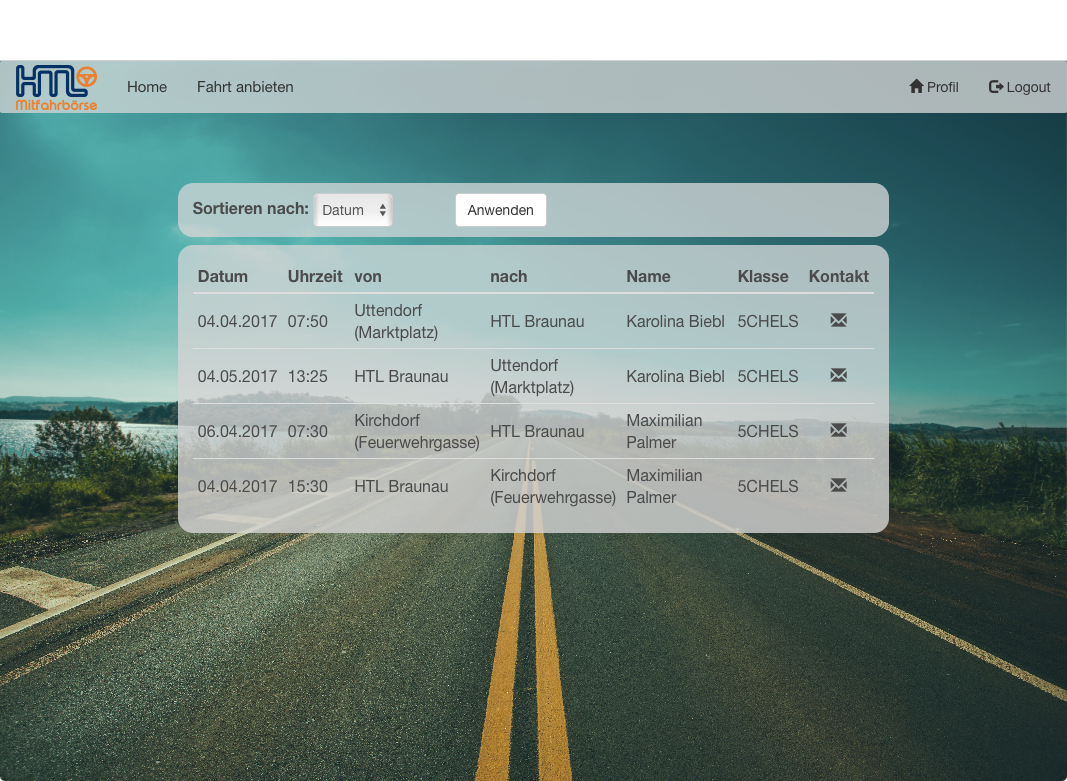
\includegraphics[width=1\linewidth]{media/images/typ_screen}
\end{center}
} \\
  
%\textbf{\mbox{Participation in} competitions, Awards} & 
%{
%Participated:
%\begin{itemize}
%\item Jugend Innovativ
%\item ITs Award
%\item FH Kärnten Maturaprojekt-Wettbewerb
%\item computer creative wettbewerb
%\item 120 Sekunden Wettbewerb
%\end{itemize}
%} \\

\textbf{\mbox{Accessibility of} \mbox{diploma thesis}} & 
{HTL Braunau archive, or\newline \url{https://diplomarbeiten.berufsbildendeschulen.at/}} \\



\end{tabularx}




%--------------------------------------------------------------------------------
% Unterschriften
%--------------------------------------------------------------------------------



\vspace*{\fill}

\textbf{Approval (date / signature)}

\fbox{
\begin{minipage}[t][3cm]{0.5\linewidth}
\centering
Examiner \\
%\hspace*{\fill}\includegraphics[width=0.8\linewidth]{fig/Unterschrift}\hspace*{\fill}
\vfill
\end{minipage}}
\fbox{
\begin{minipage}[t][3cm]{0.5\linewidth}
\centering
Head of College / Department
\vfill
\end{minipage}
}

\restoregeometry



%	--------------------------------------------------------
% 	Eidesstattliche Erklärung
%	--------------------------------------------------------			
% !TEX root = ../Vorlage_DA.tex

%	########################################################
% 					Eidesstattliche Erklärung
%	########################################################


%	--------------------------------------------------------
% 	Überschrift, Inhaltsverzeichnis
%	--------------------------------------------------------
\chapter*{Statement}
%\addcontentsline{toc}{chapter}{Erklärung}


%	--------------------------------------------------------
% 	Inhalt
%	--------------------------------------------------------

I declare in lieu of oath that I have written this diploma thesis independently and without outside help, have not used sources and aids other than those stated directly and have made the sources used verbatim and in terms of content taken as such recognizable.
\vspace{3cm}

\begin{tabularx}{\textwidth}{l p{1cm} l p{1cm} X}


Braunau/Inn, \todayshort & & Alexander Voglsperger & & \hrulefill \\
\emph{Location, Date} & & \emph{Author} & & \emph{Signature} \vspace{2cm}\\ 

Braunau/Inn, \todayshort & & Simon Moharitsch & & \hrulefill \\
\emph{Location, Date} & & \emph{Author} & & \emph{Signature} \vspace{2cm}\\ 

\end{tabularx}




%	--------------------------------------------------------
% 	Inhaltsverzeichnis
%	--------------------------------------------------------			
\tableofcontents

%	--------------------------------------------------------
% 	Vorwort
%	--------------------------------------------------------	
% !TEX root = ../Vorlage_DA.tex
%	########################################################
% 							Vorwort
%	########################################################


%	--------------------------------------------------------
% 	Überschrift, Inhaltsverzeichnis
%	--------------------------------------------------------
\chapter*{Abstract}
\addcontentsline{toc}{chapter}{Abstract}


%	--------------------------------------------------------
% 	Inhalt
%	--------------------------------------------------------

Im Vorwort teilt der Bearbeiter dem Leser wichtige Tatsachen mit, die Erklärungen zu seiner Arbeit beinhalten -- z.B. die Motivation für die Bearbeitung des Themas oder besondere Schwierigkeiten bei der Bearbeitung und/oder Materialbeschaffung. 

Hier können auch Mitteilungen persönlicher Natur enthalten sein -- z.B. Dank an Institutionen/Personen für die geleistete Unterstützung. 

%	--------------------------------------------------------
% 	Zusammenfassung
%	--------------------------------------------------------		
% !TEX root = ../Vorlage_DA.tex
%	########################################################
% 							Zusammenfassung
%	########################################################


%	--------------------------------------------------------
% 	Überschrift, Inhaltsverzeichnis
%	--------------------------------------------------------
\chapter*{Summary}
\addcontentsline{toc}{chapter}{Summary}



%	--------------------------------------------------------
% 	Inhalt
%	--------------------------------------------------------
Die \emph{Zusammenfassung} oder auch \emph{Kurzfassung} soll den Inhalt der Diplomarbeit auf maximal einer halben Seite zusammenfassen.

Dieses Dokument dient als Vorlage und Beschreibung für die Dokumentation der Diplomarbeit.
Es werden Hinweise zur Erstellung einer guten Dokumentation gegeben.
Dies betrifft welchen Inhalt die Arbeit haben soll genauso wie welche Regeln eingehalten werden müssen und mit welchen technischen Mitteln das Dokument erstellt werden kann.

Beim Inhalt dieser Arbeit wurden alle grundlegenden Qualitätsregeln eingehalten und kann daher als Musterlösung gesehen werden.
Zum Erstellen wurde das Textsatzsystem \LaTeX verwendet.
Es ist vorgesehen, dass der \LaTeX Quelltext dieses Dokuments als Ausgangspunkt für die eigene Dokumentation verwendet wird.

\begin{framed}
Dieses Dokument sollte unbedingt aufmerksam gelesen werden ehe mit der eigenen Arbeit begonnen wird.
\end{framed}



\pagebreak
\pagenumbering{arabic}	% Beginn mit arabischen Seitenzahlen

%	########################################################
%
% 						Arbeit	
%
%   Diesen Abschnitt an die eigenen Erfodernisse anpassen.		
%
%
%	########################################################

%	--------------------------------------------------------
% 	INFO: General Information for SLAMS
%	-------------------------------------------------------		
% Discription of what is a SLAM and what does it

\chapter{SLAM\authorA}

\section{What is SLAM?}
SLAM is an acronym and stands for \textbf{S}iultaneous \textbf{L}ocalization \textbf{A}nd \textbf{M}apping.
\emph{\glqq SLAM is concerned with the problem of building a map of an unknown environment by a mobile robot while at the same time navigating the environment using the map. .\grqq}~\cite{slamfordummies} \newline
This problem is thus a chicken-and-egg problem because neither the map or location are known, and have to be estimated at the same time. Cameras, Ultrasonic sensors and lidar sensors are most commonly used for fetching the 2d and 3d data of the robot's surroundings. \newline
There are several algorithms out there, which try to solve this problem using algorithms and some even deep learning. Mostly they achieve an approximate map, which is done in a reasonable time span. Many popular SLAM-algorithms use methods that include \textit{particle filters}, \textit{extended Kalman filter} and \textit{Covariance intersection}\cite{slamfordummies} \cite{1678144}. \newline

% Application environments of SLAMs
\section{Application}
The biggest selling point for using SLAM implementations is pretty simple. Many places where autonomous robots may be required don't have good enough maps that are up-to-date , if the exist at all or it might be in an environment where positioning for instance GPS can't be used properly. If slams weren't be used then someone would have to go to the place and make a map. This would delay the mission and add to the costs. \newline
With a robot, that is capable of using a SLAM method to detect and locate itself in the surroundings this wouldn't be an issue. The robot could go in, generate a map that updates itself and use it to navigate around. \newline
Existing approaches that are used are in self-driving cars, unmanned aerial vehicles, autonomous underwater vehicles, planetary rovers and newer domestic robots.

% History of slams
\section{History}
The decisive work in SLAMS was tone in the research by R.C. Smith and P. Cheeseman who worked on the representation and estimation of spatial uncertainty in 1986. Another major work in this area was done by a research group with the head being \textit{Hough F. Durrant-Whyte}. Durrant-Wyhte and his group showed that answer to SLAMS lies in the nearly infinite amount of data that can be used. This lead to the motivation of finding algorithms which are trackable and approximate in a time realistic manner.\newline
Sebastian Thrun was playing.

% List and short information about  existing SLAMs
\section{Existing Methods}
There exits a big variety of SLAM methods, that try to achieve the same goal using different approaches\cite{openslam}.
Most known or popular are the following:
\begin{itemize}
    \item \underline{EKF SLAM} \newline
    Utilizes the extended Kalman filter. The algorithm  uses the likely-hood for data association.
    It was the go-to SLAM from 1990 to 2000 until Fast SLAM was introduced.
    
    \item \underline{Fast SLAM} \newline
    Works recursively  so it scales logarithmically to the scale of the landmark. It can handle much bigger landmarks than the EKF-SLAM ever could without requiring as much computing power
    
    \item \underline{ORB-SLAM} \newline
    It's a real-time SLAM library for Monocular, Stereo and RGB-D cameras. It can detect loops and relocate the camera in real-time. It uses camera trajectory and sparse 3D reconstruction to get information out of the image sequence.
    
    \item \underline{DVO-SLAM} \newline
    Implements a \textit{dense visual SLAM} system for RGB-D cameras. It's based on \textit{Dense Visual Odometry} and was extended to include frame-to-key matching with loop closure to older key-frames.
    
    \item \underline{RGB-D SLAM} \newline
    Utilizes the depth information of a RGB-D camera, e.g., Microsoft Kinect or Intel Real-Sense Cameras
    
    \item \underline{LSD-SLAM} \newline
    It's a direct monocular SLAM. It tracks the \textit{direct image alignment} and estimates geometry in form of \textit{semi-dense depth map} instead of relying on keypoints.
    
    
\end{itemize}

%	--------------------------------------------------------
% 	INFO: General information about artificial neural networks
%	-------------------------------------------------------	
% Discription of what is a Artificial Neural Networks and what does it
\chapter{Artificial Neural Networks\authorB}

\section{What is a Artificial Neural Networks?}

  \textbf{A}rtificial \textbf{N}eural \textbf{N}etworks(ANN) are inspired by biological neural networks that constitute animal brains. Important to notice is that they are not faithful models of biologic neural or cognitive phenomena. In fact most of these models are more closely related to mathematical and/or statistical models(For Example: clustering algorithms). Such systems "learn" to perform tasks by considering examples, generally without being programmed with task-specific rules. 
 
\section{Areas of Application}

 ANN are viable computational models for a wide variety of problems, including pattern classification, speech synthesis and recognition, adaptive interfaces between human and complex physical system, function approximation, associative memory, clustering, forecasting and prediction, combinatorial optimization, nonlinear system modeling, and control
 
\section{Components of an ANN}

Simplified a ANN consists of three main components. neurons, connection and the weight associated with them and the propagation function.

\subsection{Neurons}

Neurons are elementary units in an ANN. A neuron gets one ore more inputs and depending on the value of the inputs the output is set. A neuron can get its inputs from other neurons or if its at the beginning from the source of the data that needs to be processed. Depending on the Type of ANN they are placed in different structures. The output of a Neuron is a number between 0 and 1. 

\begin{figure}[H]
	\centering
	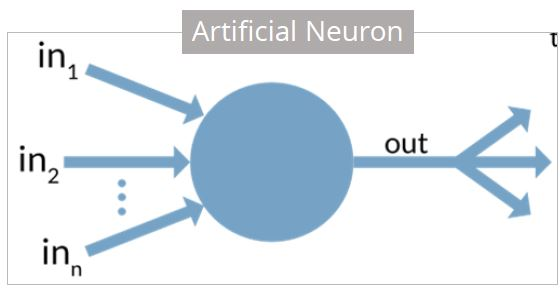
\includegraphics[width=0.7\textwidth]{./media/images/diagram-for-general-view-of-artificial-neuron.jpg}
  	\caption{General view of Neurons}
  	\label{htl01}
\end{figure}
\footnote{https://tinyurl.com/yyfthk7c}

\subsection{Connection and weights}

These Neurons are Connected. Which neurons are connected with others depends on the structure. The weights characterize how important a connection between neurons is. 

\textbf{For example:}\newline
A neuron, we call it base for this example, has two neurons connected to it as inputs. The weight of the connection of the first neuron has a bigger weight than the second connection. That means the output of the base depends more on the input of the first neuron 

\subsection{Propagation function  and activation function}

This is a function witch takes the Inputs of a neuron and the weight of these connections and adds them up. The resulting value is the processed by the activation function which sets the output.

\section{Organization}

A artificial neural network can be organized in many different ways. The following picture demonstrates a feed forward ANN 
\begin{figure}[H]
	\centering
	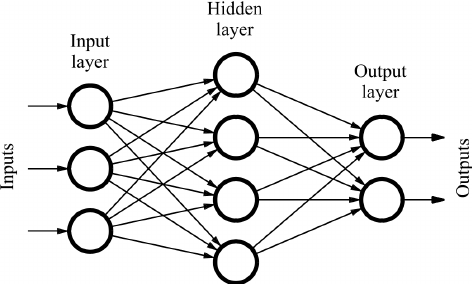
\includegraphics[width=0.7\textwidth]{./media/images/feed_forward_neural_network.png}
  	\caption{Feed forward network}
  	\label{htl01}
\end{figure}
\section{How does an ANN work?}





%	--------------------------------------------------------
% 	INFO: General information about artificial neural networks
%	-------------------------------------------------------	
% Discription of what ROS is and what it does

\chapter{Robot Operating System\authorA}

\section{What is the Robot Operating System?}
The Robot Operating System, which is also known as ROS, is a flexible framework for writing software that gets utilized on robots. ROS is a middle-ware which is not a operating system but provides services that manage hardware abstraction, low-level device control, message-passing between processes and package management. It features a collection of libraries, tools and conventions that are aimed to make the work of creating robots behaviors across a wide range of platforms more easily. \newline

\section{Design}
The processes of ROS are represented in nodes which are in a graph structure. Everything gets managed by a single process called \textit{ROS Master}, to whom all other nodes register on start. But instead of sending all of the messages over the master, the master sets up a peer-to-peer connection between the nodes. This decentralized architecture is helpful as many robots consists of many computer hardware which is connected via a network and are likely to transfer big messages.   \\
\begin{figure}[H]
	\centering
	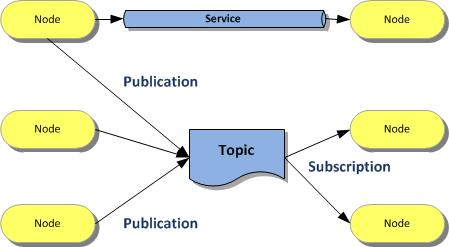
\includegraphics[width=0.7\textwidth]{./media/images/ros_structure.jpg}
  	\caption{ROS structure}
  	\label{rosstructure}
\end{figure}
\footnote{Source: https://tinyurl.com/yyfthk7c}

\subsection{Topics}
It is based on a topic system, where a topic acts like a bus over which nodes send and receive messages. Each topic must be unique in it's name, which is usually set by the developer. The process of publishing and subscribing is handles anonymously so that no node knows which nodes are sending and receiving messages on a certain topic.

\subsection{Nodes}
A node, which represent a single running process, can provide data using a matching topic and publish it to the system, where theoretically every other node can subscribe to it, to get the data. 

\section{Licenses and OS}
The language-independent tools and the main client libraries have men released under the BSD license and as such they are open source software for commercial and research use. The majority of 3rd party packages are released under several other open-source licenses.\newline
The ROS libraries are geared toward a UNIX-System which is mainly due to their dependence on a large collection of open source software and libraries.
For example \textit{Ubuntu} is in the list of supported operating systems, while others like \textit{Fedora, MacOS and Windows} are "experimental" and are mainly supported by the community.

\section{Tools}
One of the core functionalities that ROS provides are the tools which allow the developers to visualize 2D and 3D data, record data, easily navigating ROS packages, creating complex scripts that configure and setup processes. Thanks to this tools it simplifies and provides solution for common robotic development.

\subsection{Rosbag}
Rosbag is a tool that can be used over the command line to record, playback and store ROS message data. The data gets stored in a file called bag, where it records the messages as they come in. It's possible to play these bag files. By doing this the recorded messages get published into the system, as they where live. It's very handy if you need data for later development.

\subsection{CatKin}
Catkin is the newer ROS build system, which compiles the files in the source folder. It is based on CMake and is cross-platform and language-independent as most other ROS tools.

\subsection{Rviz}
A visualizer for three-dimensional data where robots, environments and sensor information can be visualized. It is highly customise able with display many types of visualisation and plugin support. \\
\begin{figure}[H]
	\centering
	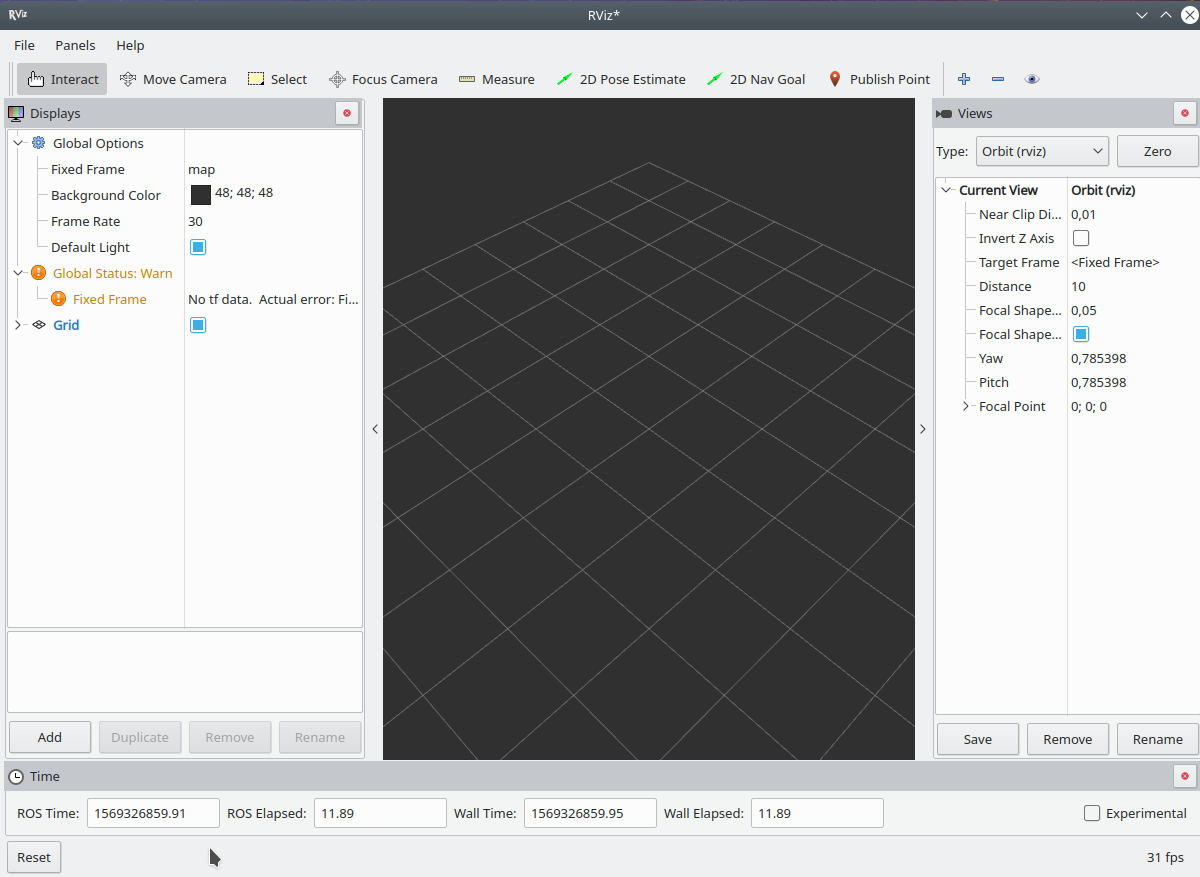
\includegraphics[width=0.7\textwidth]{./media/images/rviz}
  	\caption{Rviz interface}
  	\label{htl01}
\end{figure}

\subsection{Roslaunch}
Roslaunch is a tool for launching multiple ROS nodes and setting parameters on startup. It can be used to launch nodes locally or remotely on a server.
The configuration for a start script is written in a launch file using XML. In these files it's easy to make a automated startup and configuration process to be executed with one command. It's possible to execute launch files in other launch files to chain them together.

\subsection{RQt}
RQt provides a graphical overview of the ROS computation graph. It shows the nodes and how they are connected to each other. It also shows if a node is even subscribing to a topic or publishes something.

%	--------------------------------------------------------
% 	INFO: Gliederung und Allgemeines
%	-------------------------------------------------------	
% !TEX root = ../Vorlage_DA.tex

%	########################################################
% 			INFO: Zitieren, Abbildungen, Listing
%	########################################################


%	--------------------------------------------------------
% 	Überschrift, Inhaltsverzeichnis
%	--------------------------------------------------------
\chapter{INFO: Gliederung und Inhalt\authorB}

%	--------------------------------------------------------
\section{Gliederung}
%	--------------------------------------------------------

Die vorhergehenden Kapitel sind Muss-Bestandteile der Diplomarbeit.
Ab hier kann die Gliederung (Aufteilung in Kapitel) frei gewählt werden.

Das Dokument soll durch Kapitel und Unterkapitel übersichtlich gegliedert sein. 
Jedes Kapitel bekommt eine Überschrift mit Nummerierung (1.1, 2.2.1, ...). Mehr als 3 Überschriftebenen (1.1.1) sollten vermieden werden. Zusätzlich muss bei jedem Hauptkapitel oder Kapitel mit einer Fußnote vermerkt werden, wer diesen Abschnitt erstellt hat.

Umfangreichere Arbeitsergebnisse wie Schaltpläne, Messprotokolle, Datenblätter und das Projekttagebuch kommen in einen Anhang am Ende des Dokuments.

In einem Literaturverzeichnis sind alle verwendeten Quellen und Zitate zu sammeln.

Wird die Diplomarbeit von \textbf{mehreren Personen} gemeinsam erstellt muss erkenntlich gemacht werden wer für welches Kapitel verantwortlich war.

%	--------------------------------------------------------
\section{Beispiel Gliederung}
%	--------------------------------------------------------

Hilfestellung für eine mögliche Benennung und Gliederung der Hauptkapitel:

\begin{description}
\item[Problemanalyse und Spezifikation]
\ \\Erläuterung des \underline{Was}: Aufgabenstellung ganz detailliert (=Pflichtenheft). Hier wird erläutert, was zu machen war. Das Wie ist hier normalerweise fehl am Platz.
\item[Entwurf]
\ \\Erläuterung des Wie: Technologie mit Begründung, bzw. Abwägen der Vor- und Nachteile. Lösungswege, Algorithmen.
\item[Implementierung]
\ \\Zeigt genau die Umsetzung des Entwurfs anhand wesentlicher Quelltext-Ausschnitte.
\item[Test und Inbetriebnahme]
\ \\Erkläre wie getestet wurde und was notwendig ist um das Produkt von Null weg zu installieren.
\item[Bedienungsanleitung]
\ \\Erklärt dem Benutzer die wichtigsten Schritte bei der Bedienung des Systems.
Eventuell ist eine eigenes Bedienerhandbuch für spezielle Benutzergruppen (z.B. Administratoren) notwendig.
\item[Fazit, Schlussfolgerungen]
\ \\Hier werden die Projektergebnisse zusammengefasst. Was ist gelungen was nicht. Welche Erkenntnisse wurden gewonnen.
\item[Persönliche Erfahrungen]
\ \\Hier (und nur hier) darf subjektiv aus der Ich Perspektive über das Projekt philosophiert werden.
\end{description}


%	--------------------------------------------------------
\section{Inhalt}
%	--------------------------------------------------------

Das Ziel ist die eigene Arbeit anderen (technisch versierten, aber projektfremden) Personen nachvollziehbar zu machen.
Ein Mitschüler der ein gutes Informatik Fachwissen hat soll den Text verstehen können.

Die Dokumentation eines Informatik-Projekts soll \textbf{Programmquelltext} enthalten!
Dieser soll gut dokumentiert und lesbar sein. 
Nur wenig zusätzlicher Text soll notwendig sein um das Programm zu verstehen.
Wählt nur jene Programmteile aus, die wirklich interessant sind, nehmt nicht jene Dinge die man in jedem Buch nachlesen kann.

Werden zur Implementierung Libraries, Frameworks, Methoden, etc. verwendet die wesentlich über den normalen Unterrichtsstoff hinausgehen, so sollten diese kurz erklärt werden.
Es ist aber nicht notwendig und nicht zielführend ganze Tutorials zu erstellen.
Nach einer allgemeinen Übersicht, die zu einem grundsatzlichen Verständnis verhelfen soll, genügt es auf entsprechende Quellen zu verweisen.

Der \textbf{Umfang} der Arbeit ist nicht wesentlich, wichtig ist die Qualität des Inhalts.
Ca.\ 40 Seiten pro Person sind eine gute Richtlinie.

Der Inhalt soll aus der \textbf{eigenen Feder} stammen. 
Kopieren fremder Quellen (auch wenn diese ins Deutsche übersetzt werden müssen) ist auf ein Minimum zu beschränken. 
Wenn kopiert wird dann ist immer genau anzugeben von wo. 
Siehe auch Kapitel \ref{ref:zitieren}.

Von Dir verfasste Texte sind Deine Visitenkarte. 
Bemühe Dich alles so gut zu machen wie Du nur kannst.
\begin{itemize}
\item
Strebe nach \textbf{Perfektion} --- auch was die Rechtschreibung und Grammatik angeht.
\item
Gib keinen Text aus der Hand mit dem Du nicht 100\% zufrieden bist.
\item
Lösche unfertige Textstellen ehe Du den Text weitergibst.
\item
Suche Dir jemanden zum Korrekturlesen, in eigenen Texten übersieht man gerne Fehler die einem Anderen sofort auffallen.
\end{itemize}

Keine Erklärungen aus der \textbf{Ich-Perspektive} abgeben (Ausnahme: Fazit am Ende).

Vermeide den Text so zu schreiben wie man spricht, bei Text gelten etwas andere Regeln als bei einer Präsentation.
Verzichte auf das übernehmen mundartlicher Ausdrucksweisen.

Überlege Dir beim Schreiben einer Textstelle ob der Leser das notwendige Hintergrundwissen hat um zu verstehen was Du ausdrücken willst.
Hast Du schon vorher erklärt was man an dieser Stelle wissen sollte?
Versteht man von was die Rede ist?
Beachte, dass Du top in das Thema eingearbeitet bist. 
Was Dir völlig klar erscheint ist dem Leser vielleicht nur ein spanisches Dorf.

Sei aber auch nicht zu weitschweifig. 
Ein guter Text ist kein langer Text sondern ein Text an dem man beim besten Gewissen nichts mehr wegkürzen kann.
Schreibe zuerst etwas weitschweifiger und kürze dann radikal.
Sei nicht zimperlich, wenn Dir eine Stelle nicht gefällt, lösche diese und fange von vorne an.

 	% Nur zur Info

%	--------------------------------------------------------
% 	INFO: Zitieren, Abbildungen, Listing
%	-------------------------------------------------------	
% !TEX root = ../Vorlage_DA.tex

%	########################################################
% 			INFO: Zitieren, Abbildungen, Listing
%	########################################################


%	--------------------------------------------------------
% 	Überschrift, Inhaltsverzeichnis
%	--------------------------------------------------------
\chapter{INFO: Zitieren, Abbildungen, Quelltext\authorA}\label{ref:zitieren}

In diesem Kapitel sind Beispiele angeführt, wie Abbildungen, Zitate und Quelltext zu verwenden sind.

Die Zitate, Abbildungen und Listings werden automatisch in das Quellen- und Abbildungsverzeichnis übernommen. 
Das Literatur-, Abbildungs- und Listingsverzeichnis sind am Ende der Arbeit zu finden.   

%	--------------------------------------------------------
% 	Inhalt 
%	--------------------------------------------------------
\section{Abbildungen}\label{ref:abbildungen}

Abbildung sind mit einer Abbildungsnummer und einer Unterschrift zu versehen die kurz die Abbildung beschreibt. 
Abbildungen gehören zum umgebenden Text und müssen dort erwähnt werden.

Beispiel: In Abbildung \ref{htl01} wird das Logo der HTL Braunau dargestellt.

Wird auf eine Abbildung referenziert die sich weiter von der aktuellen Textstelle entfernt befindet so kann auch die Seitennummer hinzugefügt werden.

Beispiel: Siehe Abbildung \ref{htl01} auf Seite \pageref{htl01}.


%	--------------
%	Eine Abbildung
\begin{figure}[H]
	\centering
	
\includegraphics[width=0.5\textwidth]{./media/images/htl_c_cmyk_rein.pdf}
  	\caption{Logo der HTL Braunau.}
  	\label{htl01}
\end{figure}


%	----------------
%	Zwei Abbildungen

\begin{figure}[H]
  \centering
  \subfloat[Logo der HTL Braunau.]{\label{fig:a}
\includegraphics[width=.25\textwidth]{./media/images/htl_c_cmyk_rein.pdf}}
  \qquad
  \subfloat[Logo der HTL Braunau.]{\label{fig:b}
\includegraphics[width=.25\textwidth]{./media/images/htl_c_cmyk_rein.pdf}}
  \label{fig:canvas_01}
  % caption - In eckigen Klammern: Text für das Abbildungsverzeichnis
  \caption[Zwei Logos der HTL Braunau]{Zwei Logos der HTL Braunau in einer Abbildung zusammengefasst.}
\end{figure}


%	----------------
%	Drei Abbildungen
\begin{figure}[H]
  \centering
  \subfloat[Logo]{\label{fig:a}
\includegraphics[width=.15\textwidth]{./media/images/htl_c_cmyk_rein.pdf}}
  \qquad
  \subfloat[Logo]{\label{fig:b}
\includegraphics[width=.15\textwidth]{./media/images/htl_c_cmyk_rein.pdf}}
\qquad
  \subfloat[Logo]{\label{fig:b}
\includegraphics[width=.15\textwidth]{./media/images/htl_c_cmyk_rein.pdf}}
  \label{fig:canvas_04}
\caption[Drei Logos der HTL Braunau]{Dreimal das Logo der HTL Braunau.}
\end{figure}


\section{Zitate, Quellen, Fußnoten}

Es muss dem Leser möglich sein alle dargestellten Informationen selbst zu überprüfen.
Daher gilt der wissenschaftliche Grundsatz: 
Wer Informationen/Erkenntnisse verwendet die nicht von einem selbst stammen muss dies eindeutig kennzeichnen.
Das gilt für Bücher, Zeitschriftenartikel aber auch für alle Internetquellen.

Dem Leser Hinweise darüber zu geben wo genauere/weitere Informationen zu einem Thema zu finden sind ist ein weiterer Grund für Zitieren.

Es ist erlaubt fremde Quellen zu zitieren solange dies eindeutig erkennbar ist und sich die zitierten Stellen auf einen kurzen Absatz mit wenigen Zeilen beschränken. Auch wenn nicht wortwörtlich zitiert wird ist die Quelle der Information anzugeben.

Wörtliche Zitate werden durch Anführungszeichen begonnen und beendet sowie kursiv geschrieben: 
\emph{\glqq Wissenschaftliches Plagiat: Man kann sich zwar mit fremden Federn schmücken, aber man kann nicht mit ihnen fliegen.\grqq}~\cite{bib:uhlenbruck1}


Längere Zitate werden durch Einrücken vom normalen Text abgesetzt:
\begin{quotation}
\noindent
\emph{\glqq We tend to think of navigating a website as clicking from page-to-page via some kind of global navigation that’s always visible. When it comes to a single page, we often think scrolling is the one and only way to move from one end to the next.\grqq}~\cite{bib:bradley1}
\end{quotation}

Die eckigen Klammer mit Nummer kennzeichnet die Quelle.
Am Ende des Dokuments werden alle Quellen im Literaturverzeichnis aufgelistet. \cite{bib:wikilitverz}.

Das Verwenden fremden Gedankenguts ohne die Quelle anzugeben ist ein Plagiat (geistiger Diebstahl, \cite{bib:wikiplagiat}) und unter Umständen sogar eine Urheberrechtsverletzung.


Verweise in das Literaturverzeichnis sind nicht auf Zitate beschränkt sondern können auch eingesetzt werden um darauf hinzuweisen wo zu einem Thema mehr Informationen erhältlich sind.


Es ist zunehmend eine Kurzzitierweise in Fußnoten üblich: Nachname des Verfassers, Kurztitel, Seitenangabe.\footnote{John Doe, \glqq Verwendung von Fußnoten\grqq, Seite 12.}


%	%%%%%%%%%%%%%%%%%%%%%%%%%%%%%%%%%%%%%%%%%%%%%
%	Listings, Code
%	%%%%%%%%%%%%%%%%%%%%%%%%%%%%%%%%%%%%%%%%%%%%%
\section{Listings, Code}

Quelltext ist ein wesentlicher Bestandteil einer Informatik Diplomarbeit.
Listings werden wie Abbildungen nummeriert und mit einer Unterschrift versehen.
Ebenfalls müssen sie im Text referenziert werden.

\subsection{Beispiele}

Listing \ref{code:helloworld} auf Seite \pageref{code:helloworld} zeigt ein Hallo Welt Programm.

%	%%%%%%%%%%%%%%%%%%%%%%%%%%%%%%%%%%%%%%%%%%%%%
%	C++
\begin{minipage}{\linewidth}
\lstinputlisting[language=C++,caption={Mein erstes C-Programm.},label=code:helloworld]{./media/code_snippets/bsp_01.cpp}
\end{minipage}


Das PHP Programm \ref{code:phpread} dient zum ermitteln aller Dateien eines Unterverzeichnisses.

\begin{lstlisting}[language=PHP,caption={Alle Dateinamen ausgeben.},label=code:phpread]
<?php
if ($handle = opendir(realpath(__DIR__ . '/../userimages'))) {
    
    while (false !== ($file = readdir($handle))) {
        echo "$file//";
    }

    closedir($handle);
}
?>
\end{lstlisting}

\begin{lstlisting}[language=JavaScript,caption={Mausposition ermitteln.}]
// Calculates the mouse position.
function getMousePos(canvas, evt) {
	var rect = canvas.getBoundingClientRect();
	return {
		x: evt.clientX - rect.left,
		y: evt.clientY - rect.top
	};
}
\end{lstlisting}




%	%%%%%%%%%%%%%%%%%%%%%%%%%%%%%%%%%%%%%%%%%%%%%
%	CSS
\lstinputlisting[language=CSS,caption={Kurzer CSS--Quelltext.}]{./media/code_snippets/bsp.css}


%	%%%%%%%%%%%%%%%%%%%%%%%%%%%%%%%%%%%%%%%%%%%%%
%	HTML
\lstinputlisting[language=HTML,caption={HTML--Quelltext}]{./media/code_snippets/bsp.html}


%	%%%%%%%%%%%%%%%%%%%%%%%%%%%%%%%%%%%%%%%%%%%%%
%	HTML
\lstinputlisting[language=JavaScript,caption={JavaScript--Quelltext}]{./media/code_snippets/bsp.js}



 	% Nur zur Info

%	--------------------------------------------------------
% 	Aufgabenstellung / Pflichtenheft
%	--------------------------------------------------------		
% !TEX root = ../Vorlage_DA.tex
%	########################################################
% 				Aufgabenstellung/Pflichtenheft
%	########################################################


%	--------------------------------------------------------
% 	Überschrift, Inhaltsverzeichnis
%	--------------------------------------------------------
\chapter{Aufgabenstellung/Pflichtenheft}


%	--------------------------------------------------------
% 	Section 1
%	--------------------------------------------------------
\section{Section 1\authorA}



%	--------------------------------------------------------
% 	Section 2
%	--------------------------------------------------------
\section{Section 2\authorB}

%	--------------------------------------------------------
% 	Entwurf
%	--------------------------------------------------------	
% !TEX root = ../Vorlage_DA.tex

%	########################################################
% 				Entwurf
%	########################################################


%	--------------------------------------------------------
% 	Überschrift, Inhaltsverzeichnis
%	--------------------------------------------------------
\chapter{Entwurf}


%	--------------------------------------------------------
% 	Allgmeine Hinweise
%	--------------------------------------------------------
\section{System-Übersicht\authorA}


%	--------------------------------------------------------
% 	Lösungsansätze
%	--------------------------------------------------------
\section{Lösungsansätze\authorB}

%	--------------------------------------------------------
% 	Realisierte Lösungen
%	--------------------------------------------------------
\section{Realisierte Lösungen}


%	--------------------------------------------------------
% 	Implementierung
%	--------------------------------------------------------	
% !TEX root = ../Vorlage_DA.tex

%	########################################################
% 					Implementierung
%	########################################################


%	--------------------------------------------------------
% 	Überschrift, Inhaltsverzeichnis
%	--------------------------------------------------------
\chapter{Implementierung}


%	--------------------------------------------------------
% 	Section 1
%	--------------------------------------------------------
\section{Section 1}



%	--------------------------------------------------------
% 	Test und Inbetriebnahme
%	--------------------------------------------------------	
% !TEX root = ../Vorlage_DA.tex

%	########################################################
% 					Test und Inbetriebnahme
%	########################################################


%	--------------------------------------------------------
% 	Überschrift, Inhaltsverzeichnis
%	--------------------------------------------------------
\chapter{Test und Inbetriebnahme\authorB}


%	--------------------------------------------------------
% 	Section 1
%	--------------------------------------------------------
\section{Section 1}



%	--------------------------------------------------------
% 	Bedienungsanleitung
%	--------------------------------------------------------
% !TEX root = ../Vorlage_DA.tex
%	########################################################
% 					Bedienungsanleitung
%	########################################################


%	--------------------------------------------------------
% 	Überschrift, Inhaltsverzeichnis
%	--------------------------------------------------------
\chapter{Bedienungsanleitung\authorA}


%	--------------------------------------------------------
% 	Section 1
%	--------------------------------------------------------
\section{Section 1}



%	--------------------------------------------------------
% 	Fazit und Persönliche Erfahrungen
%	--------------------------------------------------------
% !TEX root = ../Vorlage_DA.tex

%	########################################################
% 					Fazit und Persönliche Erfahrungen
%	########################################################



%	--------------------------------------------------------
% 	Überschrift, Inhaltsverzeichnis
%	--------------------------------------------------------
\chapter{Fazit und Persönliche Erfahrungen}


%	--------------------------------------------------------
% 	Fazit
%	--------------------------------------------------------
\section{Fazit}

Zusammenfassung der Projektergebnisse. 
Besondere Erkenntnisse. Beurteilung des Lösungswegs. Eventuelle Alternativen und möglicher Erweiterungen.

%	--------------------------------------------------------
% 	Persönliche Erfahrungen
%	--------------------------------------------------------
\section{Persönliche Erfahrungen}

Hier (und nur hier) darf aus der Ich-Perspektive geschrieben werden.


%	########################################################
% 	Anhang		
%	########################################################
\appendix

%	--------------------------------------------------------
% 	Diverse Anhänge
%	--------------------------------------------------------
% !TEX root = ../Vorlage_DA.tex
%	########################################################
% 					Diverse Anhänge
%	########################################################


%	--------------------------------------------------------
% 	Überschrift, Inhaltsverzeichnis
%	--------------------------------------------------------
\chapter{Diverse Anhänge}


%	--------------------------------------------------------
% 	Projekttagebuch
%	--------------------------------------------------------
\section{Projekttagebuch}

%: TODO Grundgerüst

% http://texblog.org/2011/05/15/multi-page-tables-using-longtable/

\begin{longtable}[l]{|c|c|c|p{10cm}|}
\hline
{\scshape\bfseries Datum} & {\scshape\bfseries Schule} & {\scshape\bfseries Freizeit} & {\scshape\bfseries Tätigkeit} \\\hline\hline\endhead
22.12.2012 & 4 &  & Arbeit an der Netzwerkkommunikation.\\\hline
25.12.2012 &  & 8 & Dokumentation zu ArrayList lesen.\\\hline
\end{longtable}

Summe Schulstunden: 4\par
Summe Freizeitstunden: 8

%	--------------------------------------------------------
% 	Schaltpläne
%	--------------------------------------------------------
\section{Schaltpläne}


%	--------------------------------------------------------
% 	Quellcode
%	--------------------------------------------------------
\section{Quellcode}


%	--------------------------------------------------------
% 	Bildergalerie
%	--------------------------------------------------------
\section{Bildergalerie}


%	--------------------------------------------------------
% 	Messprotokolle
%	--------------------------------------------------------
\section{Messprotokolle}


%	--------------------------------------------------------
% 	Datenblätter
%	--------------------------------------------------------
\section{Datenblätter}	

%	--------------------------------------------------------
% 	LaTeX
%	--------------------------------------------------------	
% !TEX root = ../Vorlage_DA.tex

%	########################################################
% 					Diverse Anhänge
%	########################################################


%	--------------------------------------------------------
% 	Überschrift, Inhaltsverzeichnis
%	--------------------------------------------------------
\chapter{\LaTeX \authorA}

Das vorliegende Dokument wurde in \LaTeX\ erstellt.
\LaTeX\ (gesprochen Latech) ist ein Textsatzsystem das speziell für umfangreiche  und komplexe wissenschaftliche, technische und mathematische Dokumente entwickelt wurde.
Man schreibt Quelltext wie bei einem Programm und übersetzt diesen Quelltext in ein PDF Dokument.
Siehe \cite{bib:latexintro}.
 
%~~~~~~~~~~~~~~~~~~~~~~~~~~~~~~~~~~~~~~~~~~~~~~~~~~~~~~~~~~~~~~~~~~~~~~~~~~~~~~~~
\section{Die Vorlage}

Die \LaTeX\ Quelltexte dieses Dokuments sind gedacht um als Vorlage für die eigenen Diplomarbeit verwendet zu werden.
Dazu muss der Inhalt durch die eigene Arbeit ersetzt werden.
\verb+Vorlage_DA.tex+ ist das zentrale Haupt-Dokument, in dieses werden die einzelnen Kapitel inkludiert. Die Dateien für die eingefügten Kapitel finden sich im Unterordner \verb+chapters+.

Die Vorlage kann von GitHub geladen werden:
\url{https://github.com/matejkaf/latex-da-vorlage}

%~~~~~~~~~~~~~~~~~~~~~~~~~~~~~~~~~~~~~~~~~~~~~~~~~~~~~~~~~~~~~~~~~~~~~~~~~~~~~~~~
\section{Programme}

Programme (Editor + PDF Compiler) für \LaTeX:

Für Mac: MacTeX
\url{https://tug.org/mactex/}

Für Windows: MiKTeX
\url{http://miktex.org}\\
Zusätzlich auch die neueste Adobe Reader Version installieren!

Online:
Mit dem Service "`Overleaf"' (\url{https://www.overleaf.com/}) gab es positive Erfahrungen. Damit können die Dokument online erstellt und gemeinsam verwendet werden.



%~~~~~~~~~~~~~~~~~~~~~~~~~~~~~~~~~~~~~~~~~~~~~~~~~~~~~~~~~~~~~~~~~~~~~~~~~~~~~~~~
\section{Bitmap Fonts}


Bei MiKTeX unter Windows kann es ein Font Problem geben.
Falls die Schrift nicht scharf ist --- PDF so vergrößern dass ein Buchstabe gut 10 cm groß ist --- dann sieht man die Pixel, siehe Abbildung \ref{fig:bitmapfont}.
In diesem Fall wird ein sogenannter Bitmap-Font verwendet. 
Besser ist ein Vektor-Font, dieser lässt sich beliebig ohne Qualitätsverlust vergrößern.

\textbf{Lösung:}
Mit "`MiKTex Package Manager"' das Package \verb+cm-super+ installieren.

\begin{figure}[H]
	\centering
	
\includegraphics[width=0.75\textwidth]{./media/images/bitmap_font}
  	\caption{Oben Bitmap-, unten Vektor-Font}
  	\label{fig:bitmapfont}
\end{figure}

%~~~~~~~~~~~~~~~~~~~~~~~~~~~~~~~~~~~~~~~~~~~~~~~~~~~~~~~~~~~~~~~~~~~~~~~~~~~~~~~~
\section{LaTeX Quelltext}

Bei LaTeX wird der Text, dessen Gliederung in die Formatierung in puren Textfiles mit der Endung \verb+.tex+ beschrieben.
Die Zeichenkodierung der Files muss UTF-8 sein.

Der "`LaTeX Compiler"' (Programm mit dem Namen pdflatex) übersetzt diese Files in ein PDF Dokument.

%~~~~~~~~~~~~~~~~~~~~~~~~~~~~~~~~~~~~~~~~~~~~~~~~~~~~~~~~~~~~~~~~~~~~~~~~~~~~~~~~
\section{Gerüst}

Die Grundstruktur eines \LaTeX\ Dokuments:
\begin{Verbatim}[frame=single]
\documentclass[a4paper,10pt,final,oneside]{scrartcl}	

\usepackage{anysize}
\usepackage[utf8]{inputenc}
\usepackage[T1]{fontenc}
\usepackage[ngerman]{babel}
\usepackage[pdftex]{hyperref}
\usepackage{url}
 
\begin{document}

Ab hier kommt der Inhalt

\end{document}
\end{Verbatim}

Hinweis:
Durch die Vorlage ist diese Grund-Struktur bereits vorgegeben.

%~~~~~~~~~~~~~~~~~~~~~~~~~~~~~~~~~~~~~~~~~~~~~~~~~~~~~~~~~~~~~~~~~~~~~~~~~~~~~~~~
\section{Formatierungen}

\begin{minipage}[t]{0.6\linewidth}
\begin{Verbatim}[frame=single]
Mehrere     Leerzeichen werden 
ignoriert
ein einfacher Zeilenumbruch gilt 
als Leerzeichen.

Eine leere Zeile kennzeichnet einen 
neuen Absatz.
\end{Verbatim}
\end{minipage}
\begin{minipage}[t]{0.4\linewidth}
Mehrere     Leerzeichen werden ignoriert
ein einfacher Zeilenumbruch 
gilt als Leerzeichen.

Eine leere Zeile kennzeichnet 
einen neuen Absatz.
\end{minipage}

\vspace{1em}\noindent
Diverse Formatierungen:

\begin{tabular}{l|l}
\texttt{Typewriter} & \lstinline!\texttt{...}! o.\ \lstinline!{\ttfamily ...}!\\ 
\textbf{Fett} & \lstinline!\textbf{...}! o.\ \lstinline!{\bfseries ...}!\\ 
\textit{Italic} & \lstinline!\textit{...}! o.\ \lstinline!{\itshape ...}!\\ 
\textsl{Slanted} & \lstinline!\textsl{...}! o.\ \lstinline!{\slshape ...}!\\ 
\textsc{Kapitälchen} & \lstinline!\textsc{...}! o.\ \lstinline!{\scshape ...}!\\ 
\textmd{Normal} & \lstinline!\textmd{...}! o.\ \lstinline!{\mdseries ...}!\\ 
\emph{Emph} & \lstinline!\emph{...}! o.\ \lstinline!{\em ...}!\\ 
\textsf{Sans Serif} & \lstinline!\textsf{...}! o.\ \lstinline!{\sffamily ...}!\\
\underline{Unterstrichen} & \lstinline!\underline{...}!\\
Größen & \lstinline!\tiny! \lstinline!\scriptsize! \lstinline!\footnotesize! \lstinline!\small! \lstinline!\normalsize! \lstinline!\large! \lstinline!\Large!\\
 & \lstinline!\LARGE! \lstinline!\huge! \lstinline!\Huge!\\ 
Zentriert & \lstinline!\begin{center}...\end{center}!\\
Gesch.\ Leerz. & \lstinline!~!\\
Zeilenumbruch & \lstinline!\\! oder \lstinline!\newline!\\
Absatzumbruch & \lstinline!\par! oder leere Zeile.\\

\end{tabular}


%~~~~~~~~~~~~~~~~~~~~~~~~~~~~~~~~~~~~~~~~~~~~~~~~~~~~~~~~~~~~~~~~~~~~~~~~~~~~~~~~
\section{Überschriften}

\begin{Verbatim}[frame=single]
\chapter{Hauptkapitel}
\section{Kapitel}
\subsection{Unterkapitel}
\subsubsection{Unterunterkapitel}
\end{Verbatim}

Die Kapitelnummerierung und das Inhaltsverzeichnis werden automatisch erstellt.

%~~~~~~~~~~~~~~~~~~~~~~~~~~~~~~~~~~~~~~~~~~~~~~~~~~~~~~~~~~~~~~~~~~~~~~~~~~~~~~~~
\section{Autoren\authorB}

Für eine Diplomarbeit mit mehreren Autoren muss nachvollziehbar sein wer für welchen Teil der Urheber ist.
Dies ist durch \textbf{Namenskürzel} (2-stellig) in den Überschriften darzustellen (siehe in diesem Dokument).

Eine Person soll immer für ein komplettes Hauptkapitel (\verb+chapter+) oder Kapitel (\verb+section+) verantwortlich sein. 
Eine Aufteilung auf Ebene der Unterkapitel (\verb+subsection+) oder Unterunterkapitel (\verb+subsubsection+) sollte vermieden werden.

Die Namenskürzel werden in \verb+Vorlage_DA.tex+ definiert:

\begin{Verbatim}[frame=single]
% Initialen der Authoren
\def\authorInitialsA{MM} % Max Mustermann
\def\authorInitialsB{FF} % Frieda Fröhlich
\def\authorInitialsC{FE} % Fritz Einstein
\def\authorInitialsD{WA} % Weiterer Autor
\end{Verbatim}
 

Für das Einfügen der Namenskürzel ins Dokument dienen in weiterer Folge die Befehle 
\verb+\authorA+, 
\verb+\authorB+, 
\verb+\authorC+, 
\verb+\authorD+.

Beispiel --- erzeugt die Überschrift dieses Kapitels:
\begin{Verbatim}[frame=single]
\section{Autoren\authorB}
\end{Verbatim}

%~~~~~~~~~~~~~~~~~~~~~~~~~~~~~~~~~~~~~~~~~~~~~~~~~~~~~~~~~~~~~~~~~~~~~~~~~~~~~~~~
\section{Bilder einfügen}

Formate: pdf, jpg und png.
Dateien im Verzeichnis \verb+media/images+ ablegen.

\begin{Verbatim}[frame=single]
In Abbildung \ref{fig:htl01} sieht man das Logo der HTL Braunau.
\begin{figure}[H]
  \centering
  
\includegraphics[width=0.3\textwidth]{./media/images/htl_c_cmyk_rein.pdf}
  \caption{Logo der HTL Braunau.}
  \label{fig:htl01}
\end{figure}
\end{Verbatim}

\begin{framed}
In Abbildung \ref{fig:htl01} sieht man das Logo der HTL Braunau.
\begin{figure}[H]
	\centering
	
\includegraphics[width=0.3\textwidth]{./media/images/htl_c_cmyk_rein.pdf}
  	\caption{Logo der HTL Braunau.}
  	\label{fig:htl01}
\end{figure}
\end{framed}

Hinweis: Dateipfade mit \verb+"/"+ bilden!

Siehe
\url{http://en.wikibooks.org/wiki/LaTeX/Importing_Graphics}

Der Befehl \lstinline{\label} gibt der Abbildung einen eindeutigen Namen.
Durch \lstinline{\ref} wird dieser Name referenziert, d.h. es wird die automatisch generierte Abbildungsnummer eingefügt (dazu muss das \LaTeX\ Dokument 2-mal erstellt werden!)

Siehe \ref{ref:abbildungen}, Seite \pageref{ref:abbildungen} für Abbildungen die mehrere Bilder enthalten.

%~~~~~~~~~~~~~~~~~~~~~~~~~~~~~~~~~~~~~~~~~~~~~~~~~~~~~~~~~~~~~~~~~~~~~~~~~~~~~~~~
\section{Querverweise}

Mit Hilfe von Querverweisen verweist man auf andere Stellen im Dokument. 
Z.B. in der Form: "`Siehe \ref{ref:abbildungen}"' --- es wird die Kapitelnummer bzw. Abbildungsnummer angegeben.

Es kann auf Abbildungen und auf Überschriften verwiesen werden.
Diese erhalten zuerst mit \lstinline{\label} einen Namen.
\begin{Verbatim}[frame=single]
\section{Kapitelname} \label{ref:meinebezeichnung}
\end{Verbatim}

Möchte man auf diese Elemente verweisen gibt man den Namen im \lstinline{\ref} Befehl an.
\begin{Verbatim}[frame=single]
Eine genaue Beschreibung dieses Themas ist 
in Kapitel \ref{ref:meinebezeichnung} zu finden.
\end{Verbatim}

Ein Doppelpunkt als Teil des Namens ist erlaubt. Auf diese Weise können zum Beispiel Namen von Abbildungen, Überschriften und Listings unterschieden werden (\mbox{\lstinline{fig:}/\lstinline{ref:}/\lstinline{code:}}).

\LaTeX\ macht aus Querverweisen automatisch PDF Links.


%~~~~~~~~~~~~~~~~~~~~~~~~~~~~~~~~~~~~~~~~~~~~~~~~~~~~~~~~~~~~~~~~~~~~~~~~~~~~~~~~
\section{Aufzählungen}

\begin{minipage}[c]{0.3\linewidth}
\begin{Verbatim}[frame=single]
\begin{itemize}
\item Eins
\item Zwei
\item Drei
\end{itemize}
\end{Verbatim}
\end{minipage}
\begin{minipage}[c]{0.5\linewidth}
\begin{itemize}
\item Eins
\item Zwei
\item Drei
\end{itemize}
\end{minipage}

\noindent
\begin{minipage}[c]{0.3\linewidth}
\begin{Verbatim}[frame=single]
\begin{enumerate}
\item Eins
\item Zwei
\item Drei
\end{enumerate}
\end{Verbatim}
\end{minipage}
\begin{minipage}[c]{0.5\linewidth}
\begin{enumerate}
\item Eins
\item Zwei
\item Drei
\end{enumerate}
\end{minipage}

%~~~~~~~~~~~~~~~~~~~~~~~~~~~~~~~~~~~~~~~~~~~~~~~~~~~~~~~~~~~~~~~~~~~~~~~~~~~~~~~~
\section{Mathematische Formeln}

\begin{Verbatim}[frame=single]
Abgesetzte Formel:
\begin{equation*}
\frac{1+x}{1-x} \cdot \sqrt[3]{2} \cdot \binom{n}{k}
\end{equation*}
\end{Verbatim}

Abgesetzte Formel:
\begin{equation*}
\frac{1+x}{1-x} \cdot \sqrt[3]{2} \cdot \binom{n}{k}
\end{equation*}

\begin{Verbatim}[frame=single]
Formel im Textfluss:
$\frac{1+x}{1-x}, \sqrt[3]{2}, \binom{n}{k}$
\end{Verbatim}

Formel im Textfluß: $\frac{1+x}{1-x}, \sqrt[3]{2}, \binom{n}{k}$
\\

%~~~~~~~~~~~~~~~~~~~~~~~~~~~~~~~~~~~~~~~~~~~~~~~~~~~~~~~~~~~~~~~~~~~~~~~~~~~~~~~~
\section{Programm Quelltext}

Die Umgebung lstlisting übernimmt das Formatieren von Programmquelltext.

\begin{minipage}[t]{\linewidth}
\begin{Verbatim}[frame=single]
Listing \ref{code:complex} zeigt die Implementierung eines 
besonders komplexen Algorithmus.
\begin{lstlisting}[
    language=java,
    caption={Komplizierter Quelltext.},
    label=code:complex
]
while(x>0) {
	x--;
	// bla bla
}
\end{lstlisting}
\end{Verbatim}
\end{minipage}

\begin{framed}
Listing \ref{code:complex} zeigt die Implementierung eines 
besonders komplexen Algorithmus.
\begin{lstlisting}[
    language=java,
    caption={Komplizierter Quelltext.},
    label=code:complex
]
while(x>0) {
	x--;
	// bla bla
}
\end{lstlisting}
\end{framed}

Siehe auch \url{https://en.wikibooks.org/wiki/LaTeX/Source_Code_Listings}

%~~~~~~~~~~~~~~~~~~~~~~~~~~~~~~~~~~~~~~~~~~~~~~~~~~~~~~~~~~~~~~~~~~~~~~~~~~~~~~~~
\section{Code im Text}

\begin{minipage}[t]{\linewidth}
\begin{Verbatim}[frame=single]
Mit dem Befehl lstinline können kurze Programmfragmente 
direkt in den Textfluss integriert werden.
Das sieht dann so aus: 
\lstinline[language=java]{labels.add("" + i)}.
Allzu lange sollten diese Programmausschnitte aber nicht sein.
\end{Verbatim}
\end{minipage}

Mit dem Befehl lstinline können kurze Programmfragmente 
direkt in den Textfluß integriert werden.
Das sieht dann so aus: 
\lstinline{labels.add("" + i)}.
Allzu lange sollten diese Programmausschnitte aber nicht sein.


%~~~~~~~~~~~~~~~~~~~~~~~~~~~~~~~~~~~~~~~~~~~~~~~~~~~~~~~~~~~~~~~~~~~~~~~~~~~~~~~~
\section{Seitenümbruche}

Ein Seitenumbruch kann mit \lstinline{\pagebreak} erzwungen werden.

Soll etwas als ganzes auf der Seite stehen und nicht umgebrochen werden, so kann dieser Teil in eine \lstinline{minipage} Umgebung eingeschlossen werden.

\begin{Verbatim}[frame=single]
\begin{minipage}{\linewidth}
In diesem Teil findet kein Seitenumbruch statt.
\end{minipage}
\end{Verbatim}

Häufig wird dies bei Programmlistings nötig sein:

\begin{Verbatim}[frame=single]
Das Listing \ref{code:codenopagebreak} ist in eine minipage 
eingebunden. Dies wirkt sich so aus, dass dieses Listing nur 
als ganzes auf der Seite steht, sollte es nicht mehr Platz 
haben wird es komplett auf die folgende Seite gesetzt und 
es entsteht ein Leerraum auf der vorhergehenden Seite.

\begin{minipage}{\linewidth}
\begin{lstlisting}[
	language=java,
	caption={Java Quelltext.},
	label=code:codeexample1
]
public void prepend(Node n) {
	n.next=start;
	start=n;
}
\end{lstlisting}
\end{minipage}
\end{Verbatim}

Das Listing \ref{code:codenopagebreak} ist in eine minipage eingebunden.
Dies wirkt sich so aus, dass dieses Listing nur als ganzes auf der Seite steht, sollte es nicht mehr Platz haben wird es komplett auf die folgende Seite gesetzt und es entsteht ein Leerraum auf der vorhergehenden Seite.

\begin{minipage}{\linewidth}
\begin{lstlisting}[
	language=java,
	caption={Java Quelltext.},
	label=code:codenopagebreak
]
public void prepend(Node n) {
	n.next=start;
	start=n;
}
\end{lstlisting}
\end{minipage}


%~~~~~~~~~~~~~~~~~~~~~~~~~~~~~~~~~~~~~~~~~~~~~~~~~~~~~~~~~~~~~~~~~~~~~~~~~~~~~~~~
\section{Quellen und Literatur}

Alle Quellen befinden sich im Dokument \verb+chapters/Post-01-literatur.tex+ .
Eine Quelle erhält mit \lstinline|\bibitem{bib:name}| einen Namen.

Im Text wird durch den Befehl \lstinline{\cite} zitiert.
Bsp.:

\begin{Verbatim}[frame=single]
Siehe \cite{bib:latexintro}.
\end{Verbatim}

\begin{framed}
Siehe \cite{bib:latexintro}.
\end{framed}



%~~~~~~~~~~~~~~~~~~~~~~~~~~~~~~~~~~~~~~~~~~~~~~~~~~~~~~~~~~~~~~~~~~~~~~~~~~~~~~~~
\section{Links}

Links können in der Form einer URL eingefügt werden.
Dies kann (in kleinerem Umfang) statt Einträgen im Literaturverzeichnis verwendet werden.

\begin{Verbatim}[frame=single]
\url{http://www.orf.at}
\end{Verbatim}
\begin{framed}
\url{http://www.orf.at}
\end{framed}

Lange URL's sehen nicht besonders gut aus. Etwa \url{https://www.youtube.com/watch?v=_vQaOvPsLko&list=PL6gx4Cwl9DGBsvRxJJOzG4r4k_zLKrnxl&index=49}.

In diesem Fall bietet es sich an solche URL's mit einem Kurz-URL-Dienst (z.B. \url{tinyurl.com}) zu verkürzen. 
Obige URL in verkürzter Form: \url{http://tinyurl.com/hqtzqan}


%~~~~~~~~~~~~~~~~~~~~~~~~~~~~~~~~~~~~~~~~~~~~~~~~~~~~~~~~~~~~~~~~~~~~~~~~~~~~~~~~
\section{Fußnoten}

\begin{Verbatim}[frame=single]
Eine Fußnote kann man einfach%
\footnote{Hier zum Beispiel}
irgendwo in den Text einfuegen.
\end{Verbatim}

Eine Fußnote kann man einfach%
\footnote{Hier zum Beispiel}
irgendwo in den Text einfügen, diese wird an das untere Ende der Seite gesetzt.


%~~~~~~~~~~~~~~~~~~~~~~~~~~~~~~~~~~~~~~~~~~~~~~~~~~~~~~~~~~~~~~~~~~~~~~~~~~~~~~~~
\section{Tabellen}

Mit der Umgebung \lstinline{tabular} bzw. erweitert: \lstinline{tabularx}.

Siehe \url{https://en.wikibooks.org/wiki/LaTeX/Tables}

%: TODO Tabellen

%~~~~~~~~~~~~~~~~~~~~~~~~~~~~~~~~~~~~~~~~~~~~~~~~~~~~~~~~~~~~~~~~~~~~~~~~~~~~~~~~
\section{Mehrspaltiger Text}

\begin{multicols}{2}

Um einen zweispaltigen Text zu erzeugen kann die \verb+multicols+ Umgebung verwendet werden

\begin{Verbatim}[frame=single]
\begin{multicols}{2}
Text in 2 Spalten
\end{multicols}
\end{Verbatim}

Hier wurde multicols verwendet um die Abbildung platzsparend neben dem Text zu platzieren.
Siehe Logo der HTL Braunau in Abbildung \ref{logoTwoCols}.

%	--------------
%	Eine Abbildung

\columnbreak
\begin{figure}[H]
	\centering
	
\includegraphics[width=0.3\textwidth]{./media/images/htl_c_cmyk_rein.pdf}
  	\caption{Logo auf der rechten Seite.}
  	\label{logoTwoCols}
\end{figure}

Um einen Spaltenumbruch an einer bestimmten Stelle zu erzwingen:
\begin{Verbatim}[frame=single]
\columnbreak
\end{Verbatim}


\end{multicols}




%	--------------------------------------------------------
% 	Abschließende Prüfungen - Diplomarbeit
%	--------------------------------------------------------	
% !TEX root = ../Vorlage_DA.tex

%	########################################################
% 					Richtlinien für Diplomarbeit
%	########################################################


%	--------------------------------------------------------
% 	Überschrift, Inhaltsverzeichnis
%	--------------------------------------------------------
\chapter{Abschließende Prüfungen - Diplomarbeit}

Anbei ein Auszug aus offizieller Information bezüglich der Diplomarbeit.

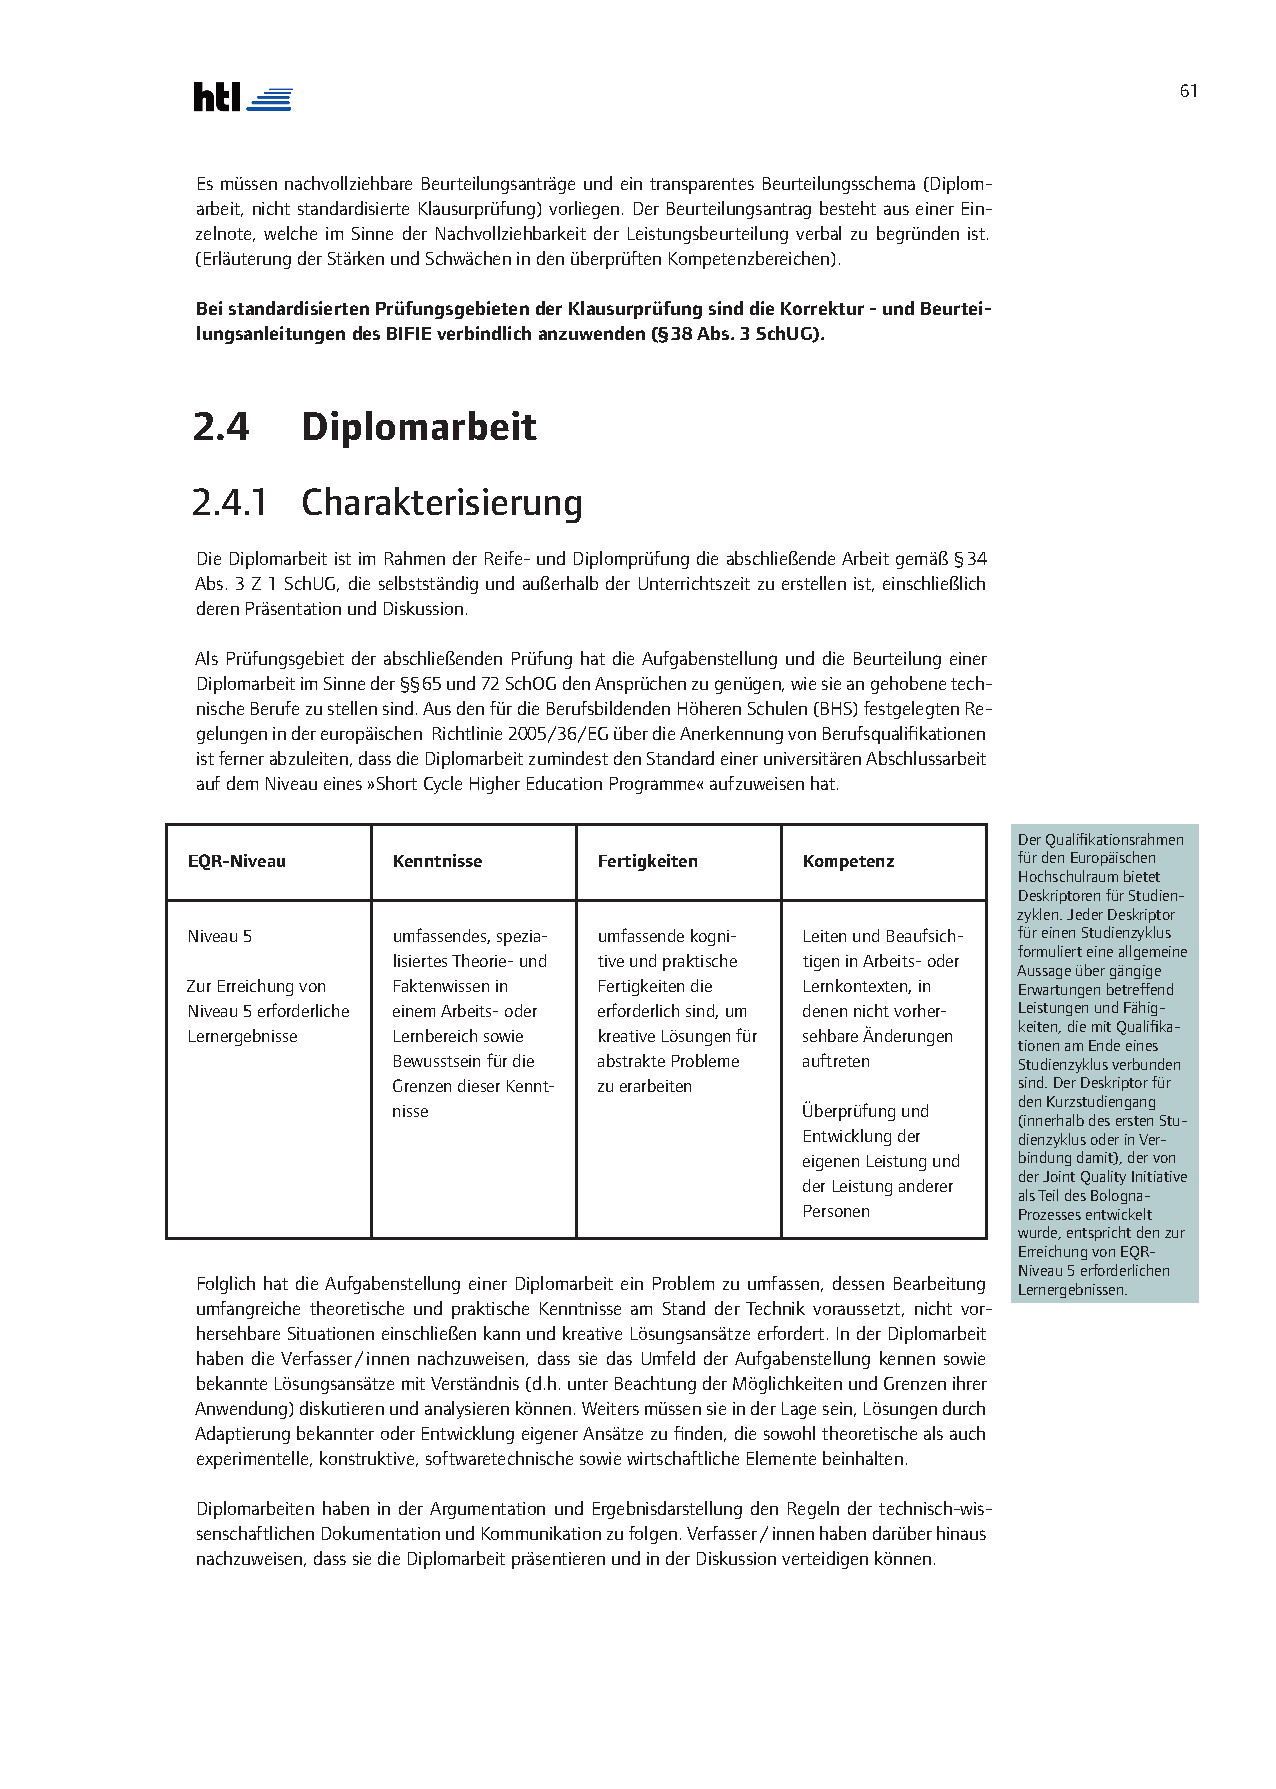
\includepdf[pages=-]{./media/info.pdf}




%	########################################################
% 	Quellenverzeichnis 		
%	########################################################
% \addcontentsline{toc}{chapter}{Literaturverzeichnis}
\bibliography{literature.bib} 
\bibliographystyle{ieeetr}

% !TEX root = ../Vorlage_DA.tex

\begin{thebibliography}{99}

\bibitem{bib:wikislam} Wikipedia,
\emph{Simultaneous localization and mapping},   \\
\url{https://en.wikipedia.org/wiki/Simultaneous_localization_and_mapping} \\
\url{https://de.wikipedia.org/wiki/Simultaneous_Localization_and_Mapping}

\bibitem{bib:techapeekslam} Scott Martin,
\emph{What is Simpultaneous Localization and Mapping},  \\
\url{https://tinyurl.com/y5yajv5u}
\

\bibitem{bib:arreverieslam} Sanket Prabhu,
\emph{Introduction to SLAM (Simultaneous Localisation and Mapping)},    \\
\url{https://tinyurl.com/y5an9jq9}

\bibitem{bib:openslam} OpenSLAM,
\emph{Existing SLAM methods},   \\
\url{https://openslam-org.github.io/}

\bibitem{bib:wikislamlist} Wikipedia,
\emph{List of SLAM methods},    \\
\url{https://en.wikipedia.org/wiki/List_of_SLAM_Methods}

\bibitem{bib:wikiekfslam} Wikipedia,
\emph{Extended Kalman Filter SLAM},    \\
\url{https://en.wikipedia.org/wiki/EKF_SLAM}

\bibitem{bib:rosrgbdslam} ROS-Wiki,
\emph{RGB-D SLAM},  \\
\url{https://wiki.ros.org/rgbdslam}

\bibitem{bib:orbslam2} Raul Mur-Artal, i.a.,
\emph{ORB-SLAM2},   \\
\url{https://github.com/raulmur/ORB_SLAM2}

\bibitem{bib:tumdvoslam} TU Munich - Vision,
\emph{Dense Visual Odometry SLAM},  \\
\url{https://vision.in.tum.de/data/software/dvo}

\bibitem{bib:tumlsdslam} TU Munich - Vision,
\emph{LSD-SLAM},    \\
\url{https://vision.in.tum.de/research/vslam/lsdslam}

\bibitem{bib:fastslam} Michael Montemerlo, i.a.,
\emph{FastSLAM: A Factored Solution to the Simultaneous Localization and Mapping Problem},   \\
\url{https://www.cs.cmu.edu/~mmde/mmdeaaai2002.pdf}

\bibitem{bib:rosabout} ROS,
\emph{About ROS},   \\
\url{https://www.ros.org/about-ros/}

\bibitem{bib:wikiros} Wikipedia,
\emph{Robot Operating System},   \\
\url{https://en.wikipedia.org/wiki/Robot_Operating_System}

\bibitem{bib:wikiann} Wikipedia,
\emph{About Artificial neural networks},   \\
\url{https://en.wikipedia.org/wiki/Artificial_neural_network}

\bibitem{bib:mohamadann} Mohamad H. Hassoun,
\emph{About Fundamentals of artificial neural networks},   \\
\url{https://tinyurl.com/y2wss5cq}

\bibitem{bib:wikineuron} Wikipedia,
\emph{About Artificial neurons},   \\
\url{https://en.wikipedia.org/wiki/Artificial_neuron}

\bibitem{bib:generelann} nnwj,
\emph{About Neural Networks},   \\
\url{https://www.nnwj.de/neural-net-components.html}

% Grafiken

\bibitem{bib:neuronimage} simplilearn,
\emph{About Artificial neurons image},   \\
\url{https://www.simplilearn.com/what-is-perceptron-tutorial}

%
%\bibitem{bib:bradley1} Steven Bradley,
%\emph{Exploration Of Single-Page Websites},
%\url{http://tinyurl.com/jgx7hf3},
%Smashing Magazine, (2012)

%
%\bibitem{bib:latexintro} T.~Oetiker, et.al., 
%\emph{The not so short introduction into LaTeX}, \\
%\url{https://tobi.oetiker.ch/lshort/lshort.pdf}

%
%\bibitem{bib:wikilitverz} Wikipedia, 
%\emph{Literaturverzeichnis}, \\
%\url{http://de.wikipedia.org/wiki/Literaturverzeichnis}

%
%\bibitem{bib:wikiplagiat} Wikipedia, 
%\emph{Plagiat}, 
%\url{http://de.wikipedia.org/wiki/Plagiat}

%
%\bibitem{bib:uhlenbruck1} Gerhard Uhlenbruck, 
%\emph{Kein Blatt vor den Mund nehmen}, 
%\url{...}, Ralf Reglin Verlag Köln (2005), ISBN 3-930620-25-1

\end{thebibliography} 






%	########################################################
% 	Abbildungsverzeichnis 		
%	########################################################
\addcontentsline{toc}{chapter}{Abbildungsverzeichnis}
\listoffigures

%	########################################################
% 	Verzeichnis der Listings 		
%	########################################################
\addcontentsline{toc}{chapter}{Quelltextverzeichnis}
\lstlistoflistings

%	--------------------------------------------------------
% 	Autoren
%	--------------------------------------------------------
% !TEX root = ../Vorlage_DA.tex
%	########################################################
% 					Autoren
%	########################################################


%	--------------------------------------------------------
% 	Überschrift, Inhaltsverzeichnis
%	--------------------------------------------------------
\chapter*{Authors} \markboth{Authors}{Authors}
\addcontentsline{toc}{chapter}{Authors}

%	--------------------------------------------------------
% 	Autor 1
%	--------------------------------------------------------
\htlParagraph{Alexander Voglsperger}

\renewcommand{\arraystretch}{1.2}
\begin{tabularx}{1\textwidth}{@{} l X l @{}}

\emph{Birthday, Place of birth:} & 25.03.2001, Ried im Innkreis & 
\multirow{5}{2.5cm}{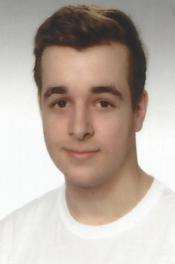
\includegraphics[width=2.5cm]{./media/images/alexander.png}
} 
\\
\emph{School education:} & Volksschule Aurolzmünster \newline Informatik Hauptschule Aurolzmünster \newline HTL Braunau & \\
\emph{Internship:} & Team7 Natürlich Wohnen GmbH, 4 Weeks, IT\newline
Krankenhaus Ried im Innkreis, 4 Weeks, IT\newline
Johannes Kepler University - AI Lab, 4 Weeks, Mapping and Tracking on self-driving car&\\
\emph{Address:} & Forchtenau 196\newline 4971, Aurolzmünster\newline Österreich & \\
\emph{E-Mail:} & alexander.voglsperger@gmail.com & \\

\end{tabularx}
\\\\

%	--------------------------------------------------------
% 	Autor 2
%	--------------------------------------------------------
\htlParagraph{Simon Moharitsch}

\begin{tabularx}{1\textwidth}{@{} l X l @{}}
\emph{Birthday, Place of birth:} & 01.01.1970, Braunau am Inn & 
\multirow{5}{2.5cm}{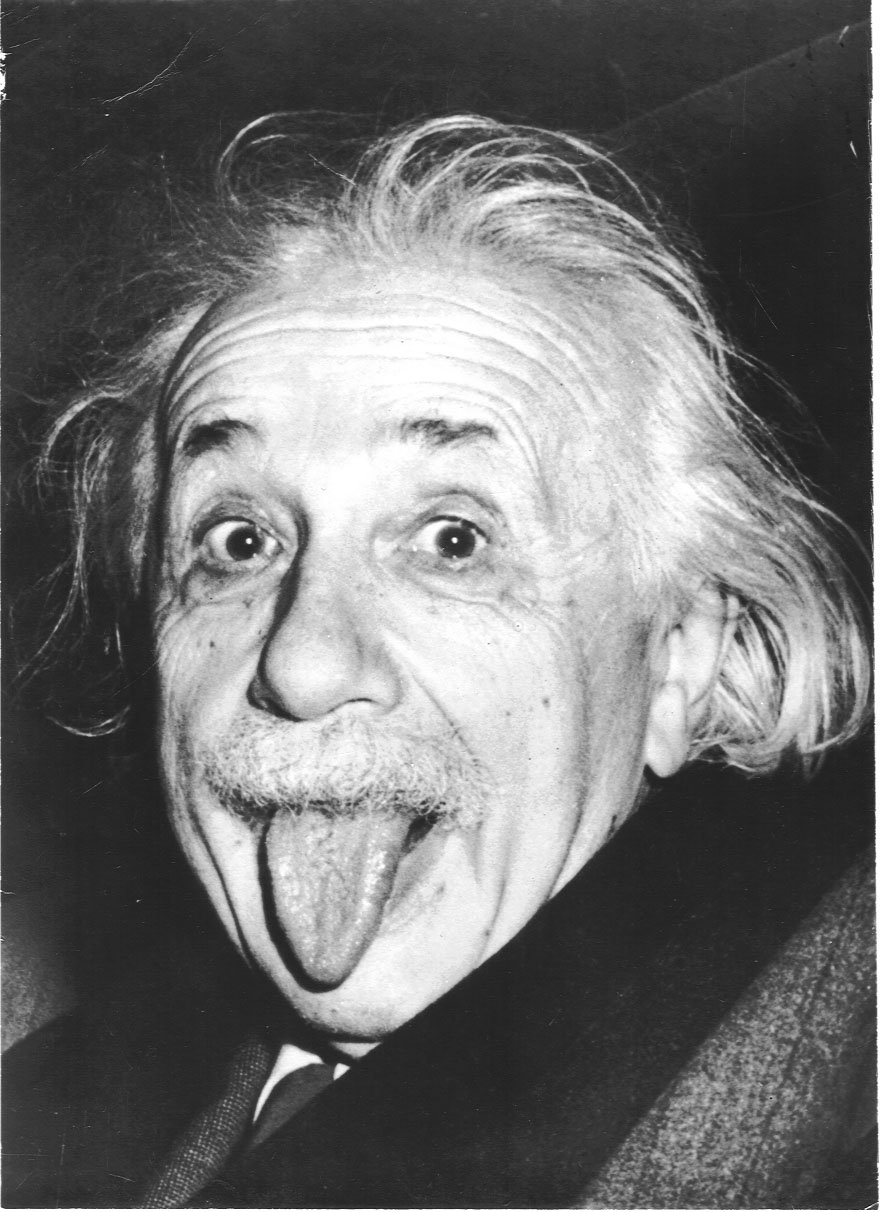
\includegraphics[width=2.5cm]{./media/images/einstein.jpg}
} 
\\
\emph{School education:} & Volksschule \newline Hauptschule \newline HTL & \\
\emph{Internship:} & Firmenname, Zeit, Tätigkeit & \\
\emph{Address:} & Strasse Nummer\newline PLZ, Ort\newline Österreich & \\
\emph{E-Mail:} & max@mustermann.com & \\

\end{tabularx}




\end{document}  